%
% PROJECT: <ETD> Electronic Thesis and Dissertation Initiative
%   TITLE: LaTeX report template for ETDs in LaTeX
%  AUTHOR: Neill Kipp, nkipp@vt.edu
%     URL: http://etd.vt.edu/latex/
% SAVE AS: etd.tex
% REVISED: September 6, 1997 [GMc 8/30/10]
% 

% Instructions: Remove the data from this document and replace it with your own,
% keeping the style and formatting information intact.  More instructions
% appear on the Web site listed above.

\documentclass[12pt]{report}

\usepackage{epsfig,endnotes}

\usepackage{color}
\usepackage{epstopdf}
\usepackage{psfrag}
\usepackage{subfigure}
\usepackage{xspace}
\usepackage{booktabs}
%\usepackage{float}
\usepackage[hyphens]{url}
\usepackage{path}
\usepackage[font=small,labelfont=bf]{caption}
\usepackage{courier}
\usepackage{listings}
\usepackage{pifont}
\usepackage{graphicx}
\usepackage{hyperref}
\usepackage{minted}
\usepackage{multirow}


\setlength{\textwidth}{6.5in}
\setlength{\textheight}{8.5in}
\setlength{\evensidemargin}{0in}
\setlength{\oddsidemargin}{0in}
\setlength{\topmargin}{0in}

\setlength{\parindent}{0pt}
\setlength{\parskip}{0.1in}

% Uncomment for double-spaced document.
\renewcommand{\baselinestretch}{1.5}

% \usepackage{epsf}

\begin{document}
\newcommand{\cb}{Cloud\-Browser\xspace}
\newcommand{\projectname}{Cloud\-Browser\xspace}
\newcommand{\cbtwo}{Cloud\-Browser 2.0\xspace}
\newcommand{\js}{Java\-Script\xspace}
\newcommand{\nodejs}{Node.js\xspace}
\newcommand{\appins}{App Instance\xspace}
\newcommand{\jsdom}{JSDOM\xspace}
\newcommand{\citemain}{~\cite{mcdaniel2012cloudbrowser}}
\newcommand{\etdtitle}{Rich Cloud-based Web Applications with \cbtwo}

%% A ``long'' caption.  Long captions show up in the list of
%% tables/figures with only the first argument.  Both arguments
%% show up in the actual caption.
\newcommand{\longcaption}[2]{\caption[#1]{#1 #2}}

\newcommand{\webscaleoutfig}{
    \begin{figure}[tb]
    \centering
    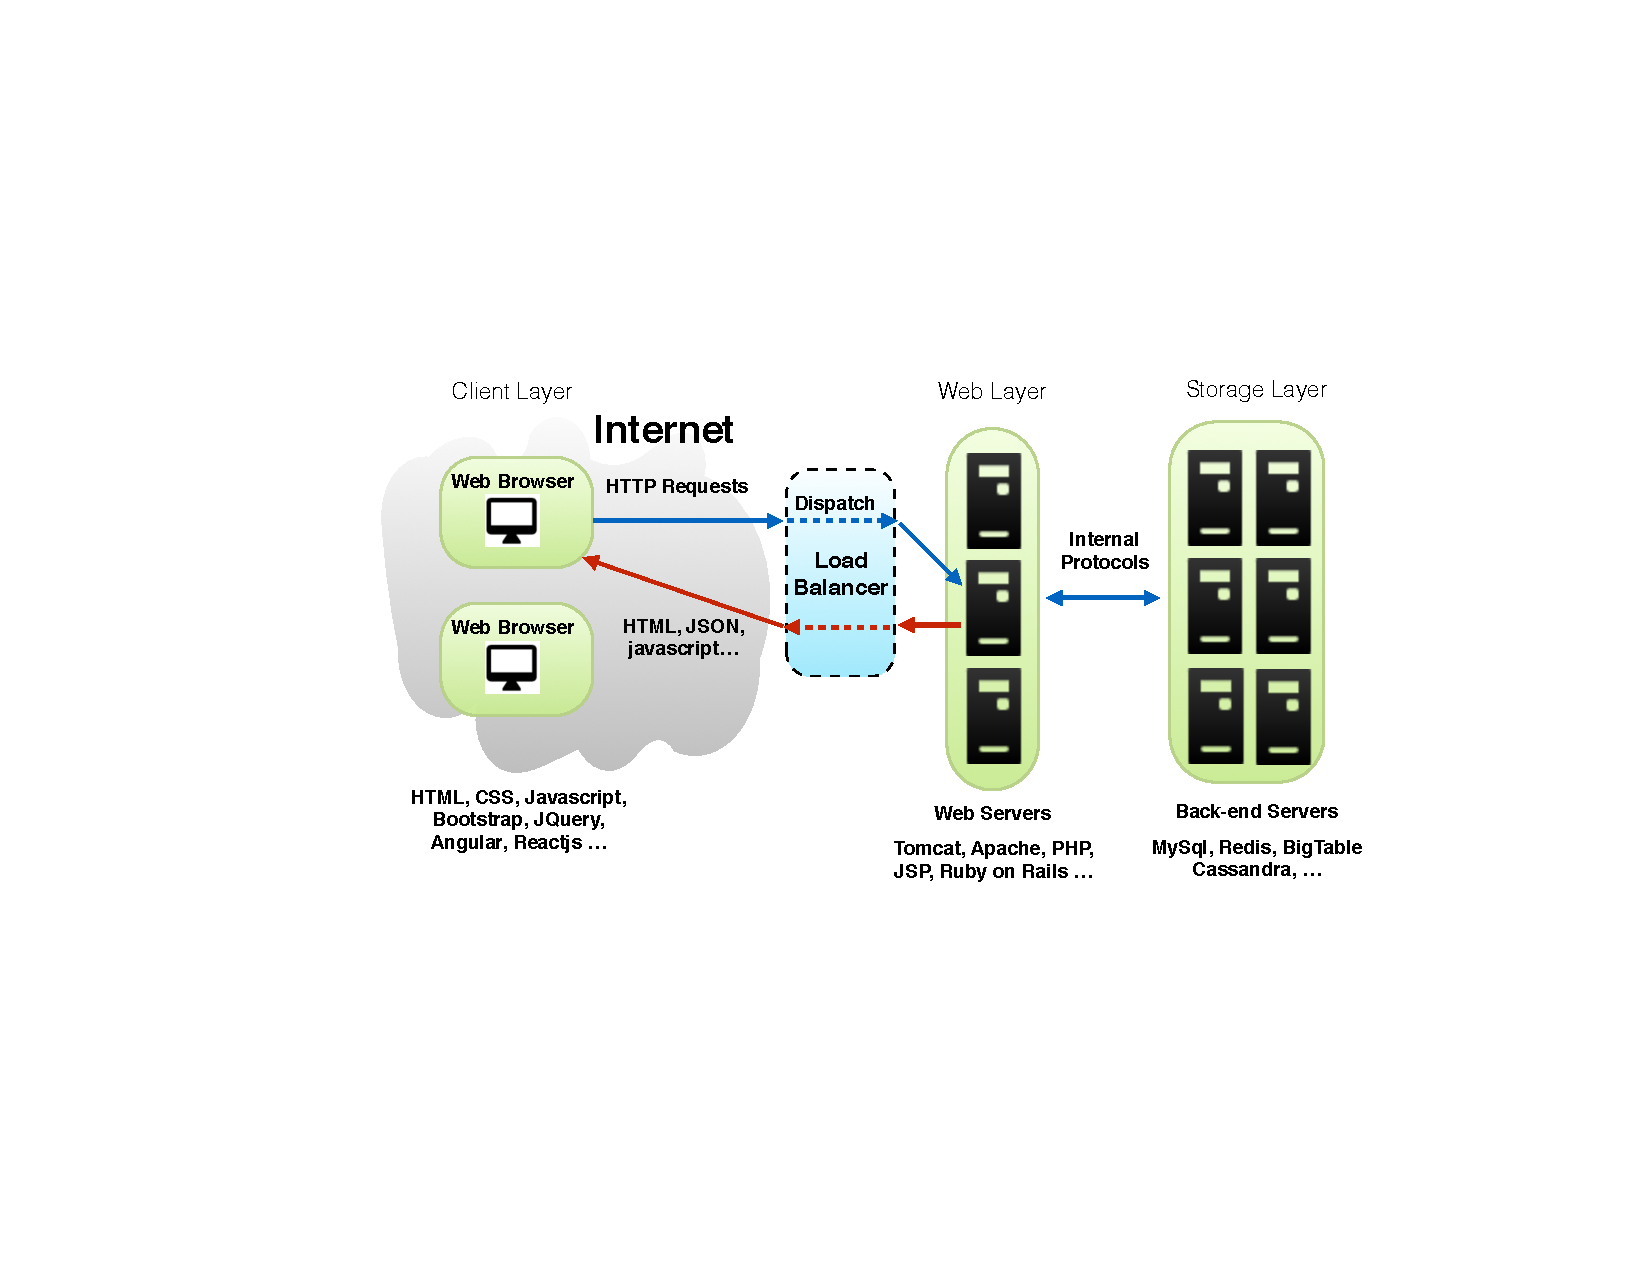
\includegraphics[width=\textwidth]{../figs/web_scale_out}
    \caption{Scalable web server architecture}
    \label{fig:webscaleout}
    \end{figure}
}

\newcommand{\architectureoverview}{
    \begin{figure*}[ht]
    \centering
    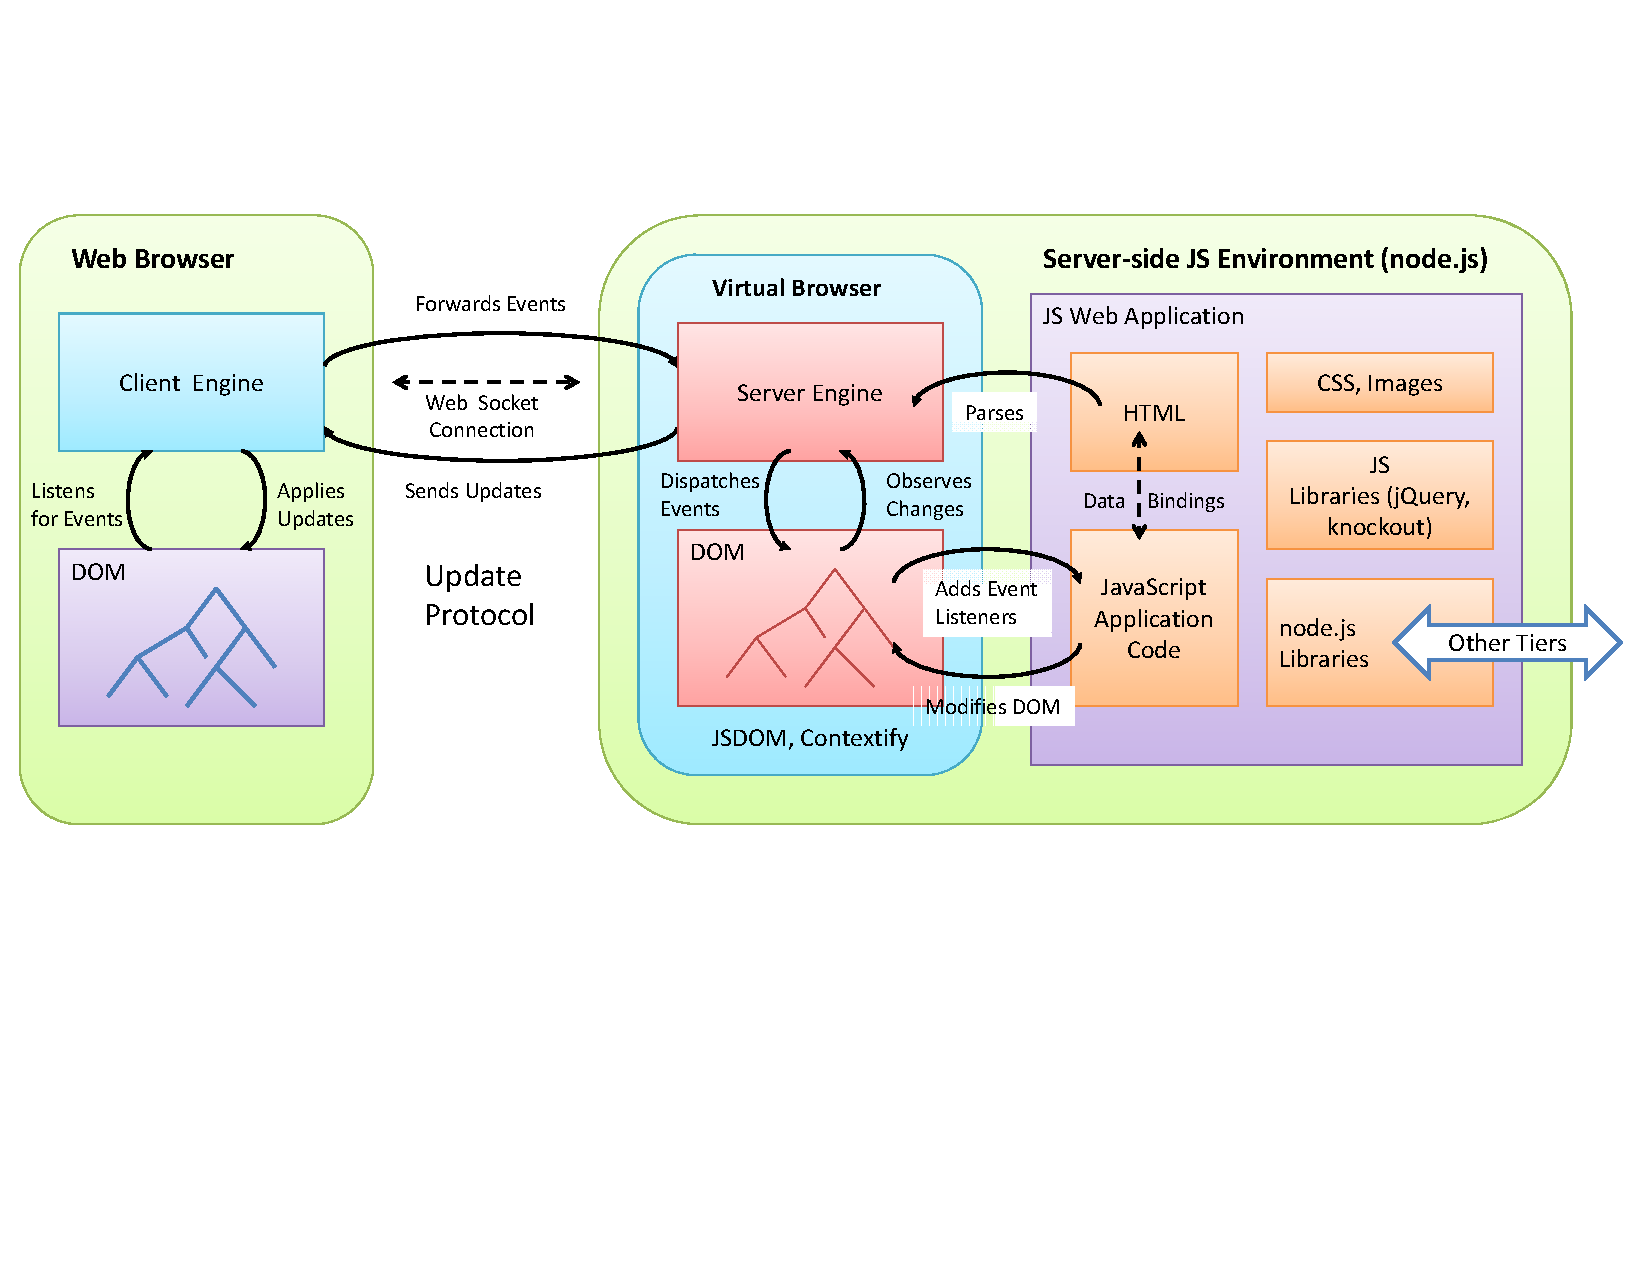
\includegraphics[width=\textwidth]{../figs/architecture_overview}
    \caption{Single Process \cb{} Architecture Overview}
    \label{fig:cb1arch}
    \end{figure*}
}

\newcommand{\newarchitectureoverview}{
    \begin{figure*}[ht]
    \centering
    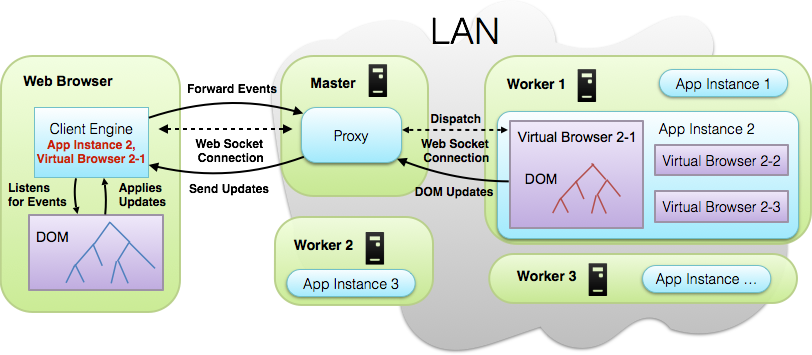
\includegraphics[width=\textwidth]{../figs/new_architecture_overview}
    \caption{Multiprocess Process \cb{} Architecture Overview}
    \label{fig:cb2arch}
    \end{figure*}
}


\newcommand{\appinstancefig}{
    \begin{figure}[ht]
    \centering
    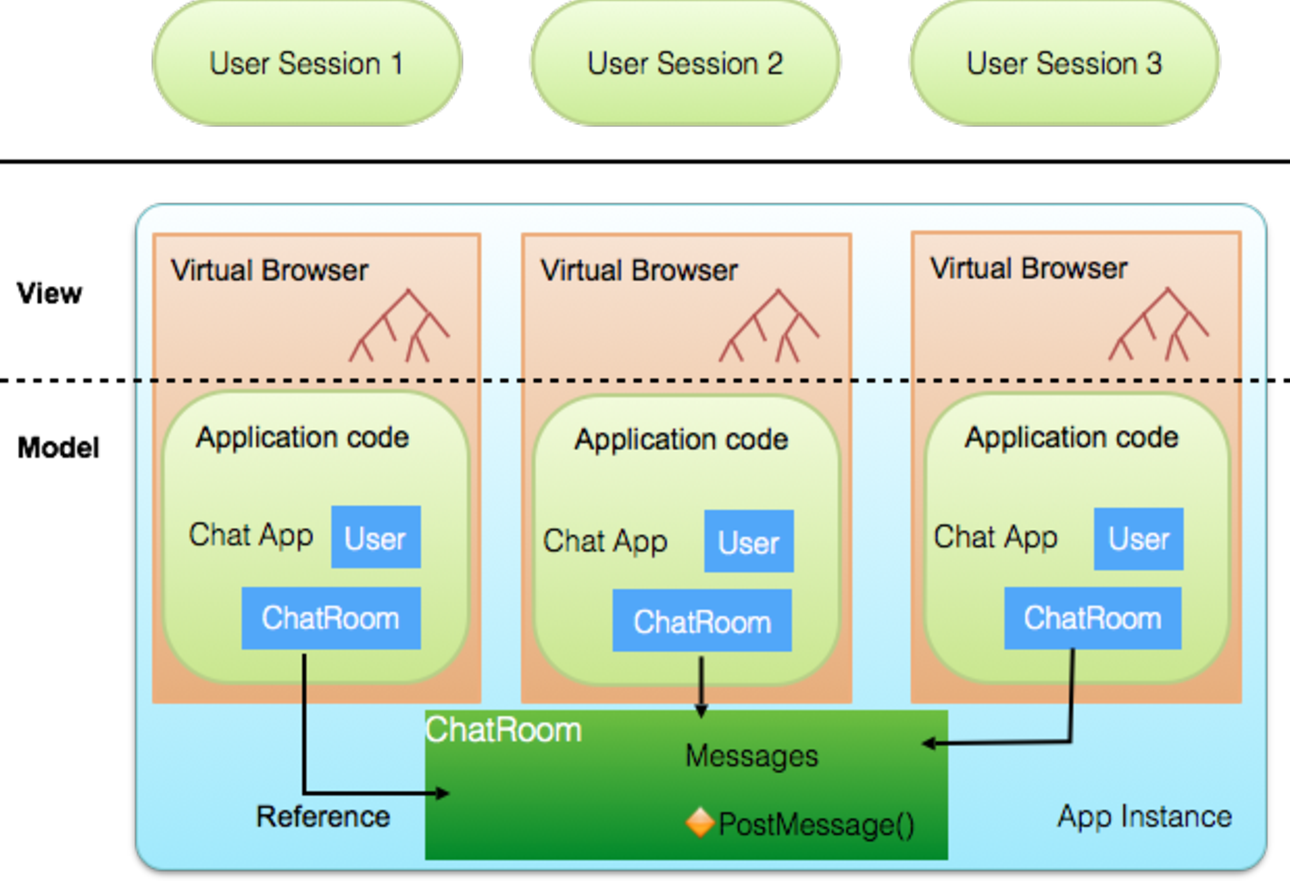
\includegraphics[width=0.8\textwidth]{../figs/appInstance}
    \caption{Application Instance}
    \label{fig:appinstance}
    \end{figure}
}


\newcommand{\appbundlefig}{
    \begin{figure}[ht]
    \centering
    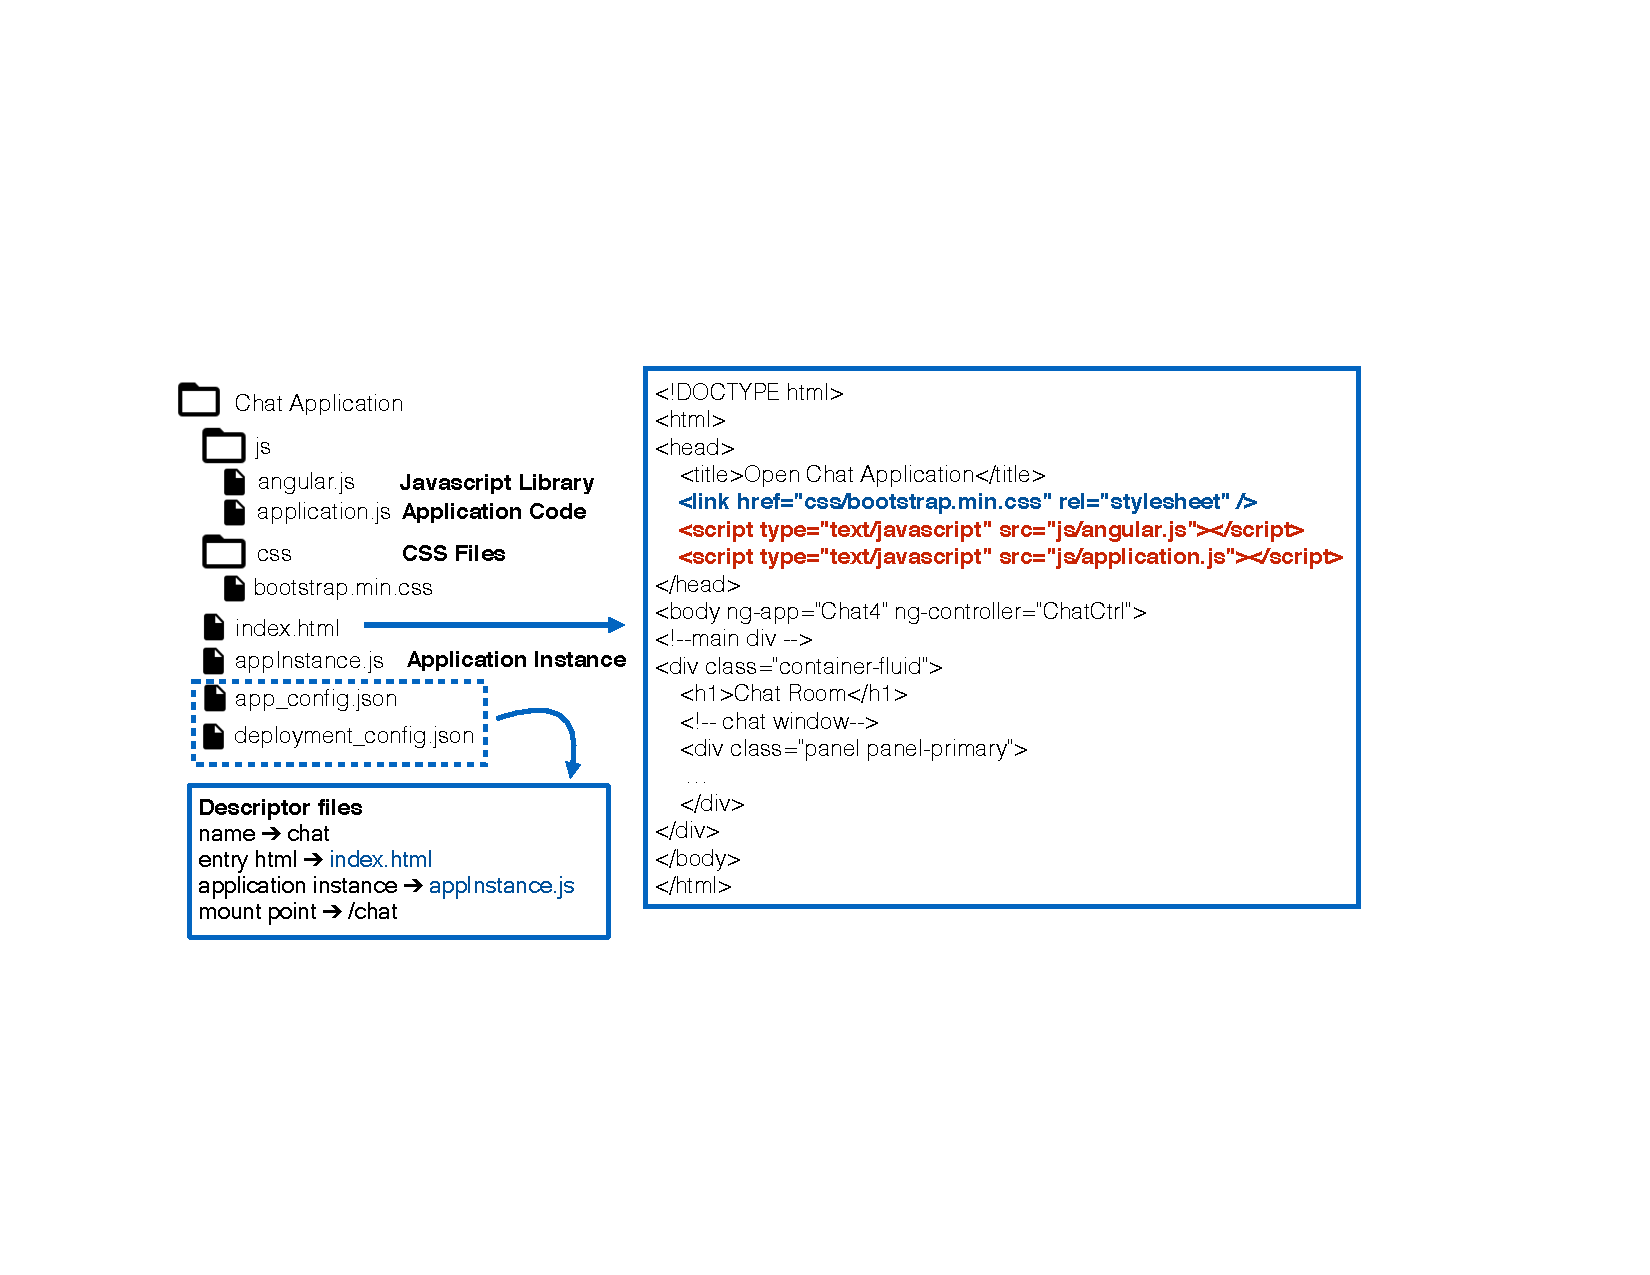
\includegraphics[width=\textwidth]{../figs/application_bundle}
    \caption{Folder structure of a \cb application}
    \label{fig:appbundle}
    \end{figure}
}

\newcommand{\chatappfig}{
    \begin{figure}[ht]
    \centering
    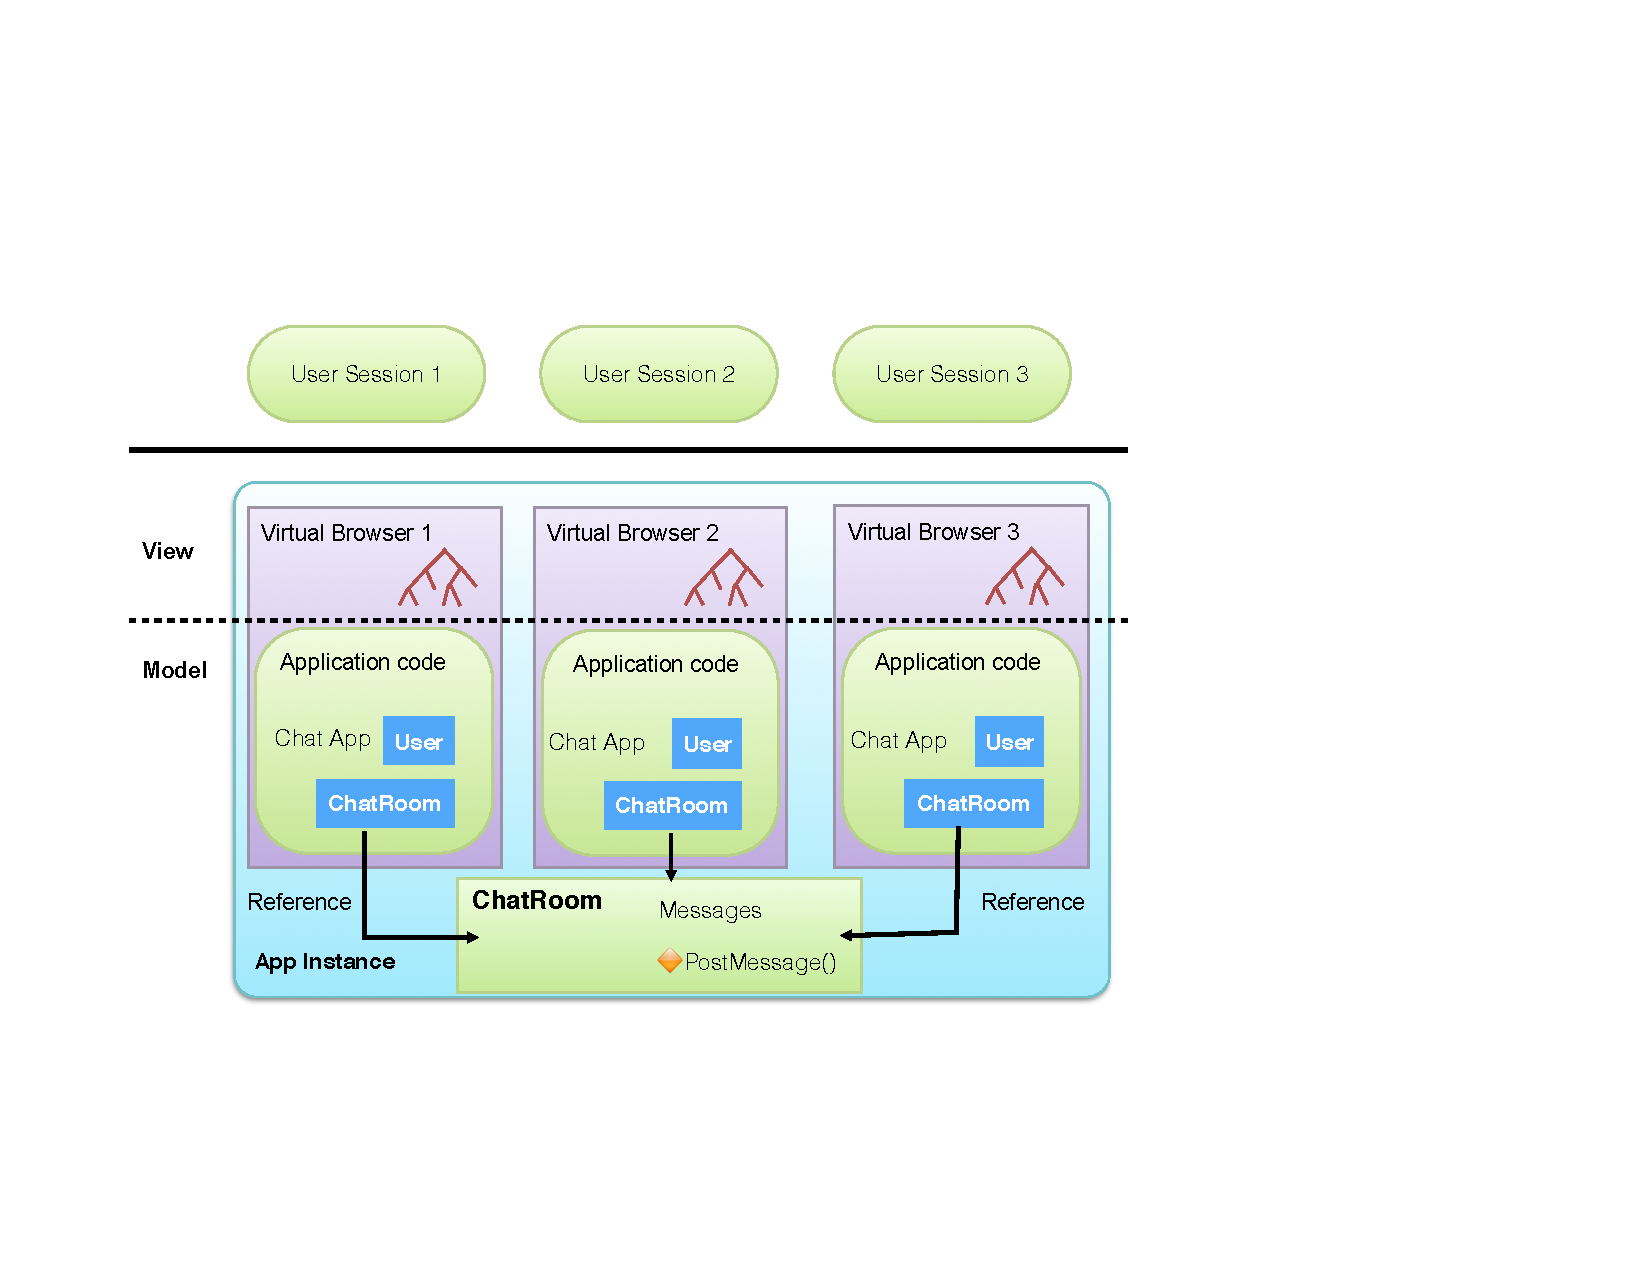
\includegraphics[width=0.8\textwidth]{../figs/chat_application}
    \caption[Sharing data among multiple virtual browser via application instance]
        {This figure shows how multiple virtual browsers can directly,
        and seamlessly share relevant application data, in this case chat messages,
        which then become part of the model that drives the presentation
        MVC framework.
    }
    \label{fig:chatapp}
    \end{figure}
}


\newcommand{\clickthroughput}{
    \begin{figure}[ht]
    \centering
    \includegraphics[width=\textwidth]{../gnuplot/click_throughput}
    \caption{Throughput of ``Back-to-back'' click application.}
    \label{fig:clickthroughput}
    \end{figure}
}


\newcommand{\clicklatency}{
    \begin{figure}[ht]
    \centering
    \includegraphics[width=\textwidth]{../gnuplot/click_latency}
    \caption{Latency of ``Back-to-back'' click application.}
    \label{fig:clicklatency}
    \end{figure}
}


\newcommand{\clickwaitthroughput}{
    \begin{figure}[ht]
    \centering
    \includegraphics[width=\textwidth]{../gnuplot/click_wait_throughput}
    \caption{Throughput of click application, after introducing artificial delay.}
    \label{fig:clickwaitthroughput}
    \end{figure}
}


\newcommand{\clickwaitlatency}{
    \begin{figure}[tb]
    \centering
    \includegraphics[width=\textwidth]{../gnuplot/click_wait_latency}
    \caption{Latency of click application, after introducing artificial delay.}
    \label{fig:clickwaitlatency}
    \end{figure}
}



\newcommand{\angularchatlatency}{
    \begin{figure}[tb]
    \centering
    \includegraphics[width=\textwidth]{../gnuplot/angularchat_latency}
    \caption{Latency of chat application with Angular.js.}
    \label{fig:angularchatlatency}
    \end{figure}
}


\newcommand{\jquerychatlatency}{
    \begin{figure}[tb]
    \centering
    \includegraphics[width=\textwidth]{../gnuplot/jquerychat_latency}
    \caption{Latency of chat application with JQuery.}
    \label{fig:jquerychatlatency}
    \end{figure}
}


\newcommand{\chatroomfig}{
    \begin{figure}[tb]
    \centering
    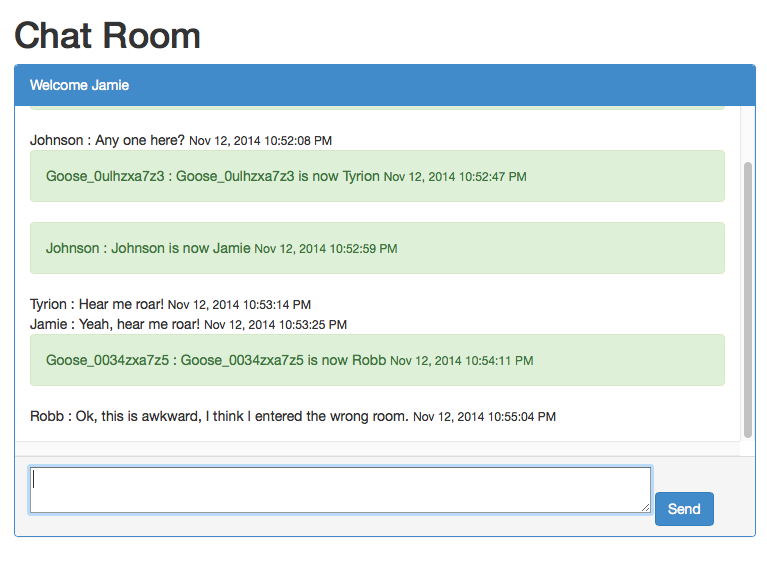
\includegraphics[width=\textwidth]{../figs/chatroom}
    \caption{Chat Room Application}
    \label{fig:chatroom}
    \end{figure}
}

\newcommand{\apphierarchyfig}{
    \begin{figure}[tb]
    \centering
    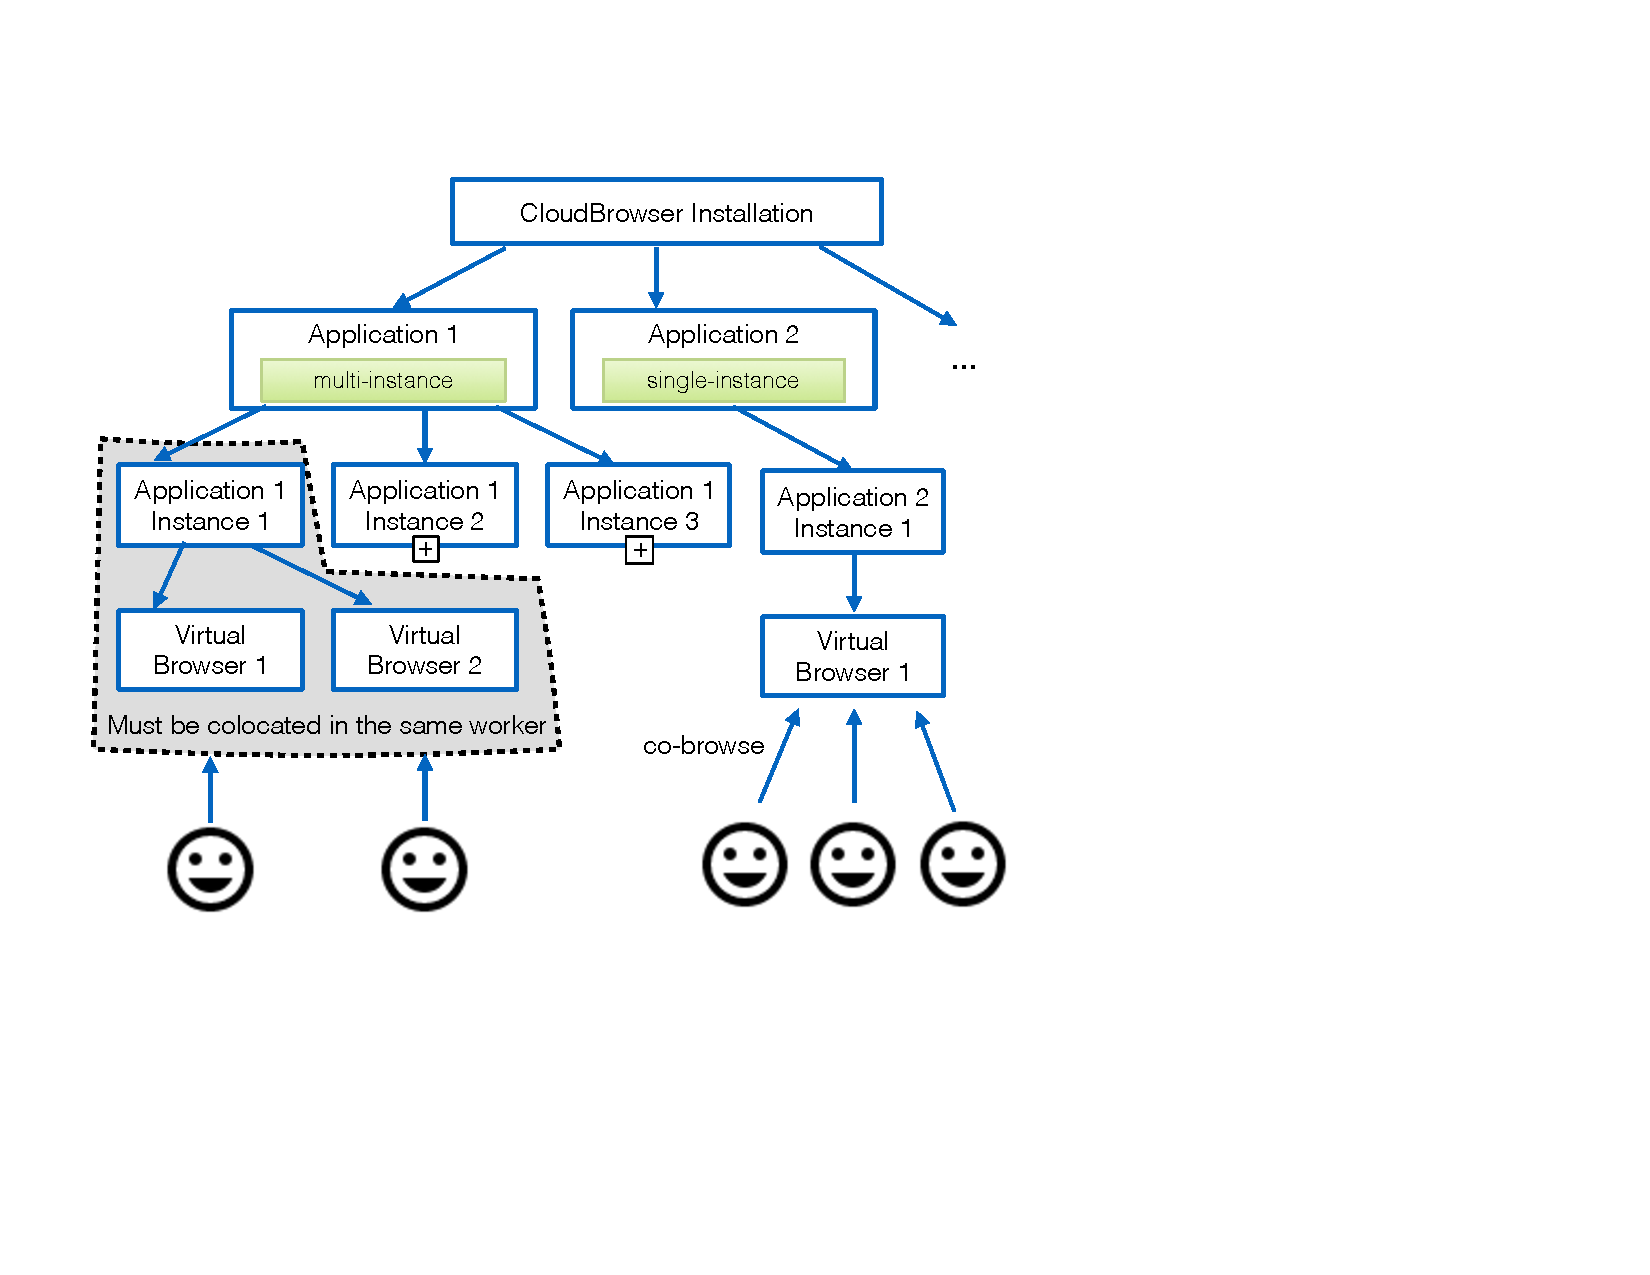
\includegraphics[width=0.8\textwidth]{../figs/application_hierarchy}
    \caption[Application deployment model]{Application deployment model: Hierarchy of applications, application instances, and virtual browsers.
    Note that a single virtual browser may be broadcast to multiple clients (cobrowsing).}
    \label{fig:appidhierarchy}
    \end{figure}
}

\newcommand{\memfig}{
\begin{figure*}[ht]
    \centering
    \includegraphics[width=\textwidth]{../gnuplot/resource_consumption}
    \caption[Resource Consumption of worker]{
    Resource Consumption of worker node running JQueryChat Application\\
X axis is time. Left Y axis corresponds to the red line of CPU usage.
Right Y axis corresponds to memory statistics.\\
After about 90s after the system boots up, the benchmark tool starts to simulate 
user workload.
When the benchmark tool sending requests, \emph{HeapUsed} fluctuates as the system creates new objects and garbage collector cleans dead objects.
When the \emph{HeapUsed} drops there is a steep surge of CPU usage, indicating garbage collector is working at that time.
    }
    \label{fig:mem}
\end{figure*}
}


\newcommand{\nodermifig}{
    \begin{figure}[ht]
    \centering
    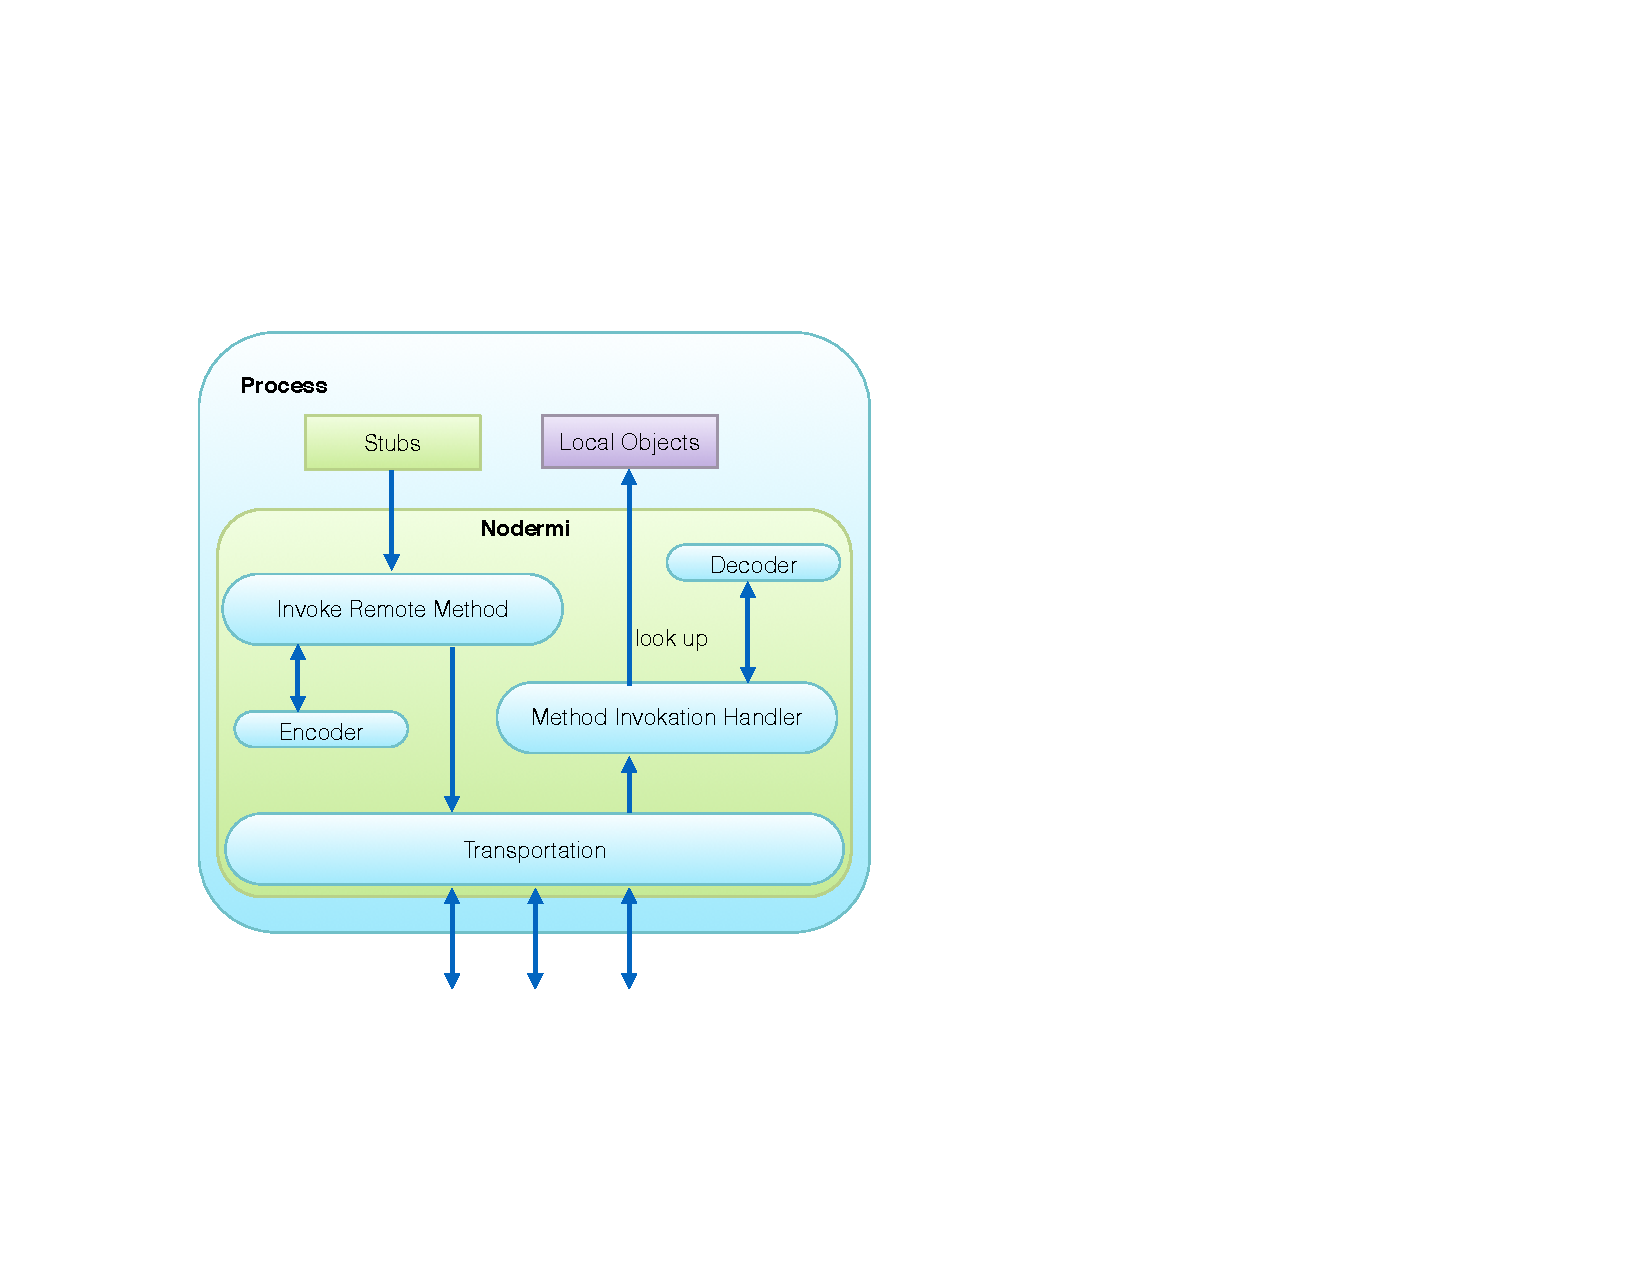
\includegraphics[width=\textwidth]{../figs/nodermi}
    \caption[Overall Design of nodermi]{Overall Design of nodermi}
    \label{fig:nodermi}
    \end{figure}
}

% deprecated
\newcommand{\nodermimethodinvokefig}{
    \begin{figure}[ht]
    \centering
    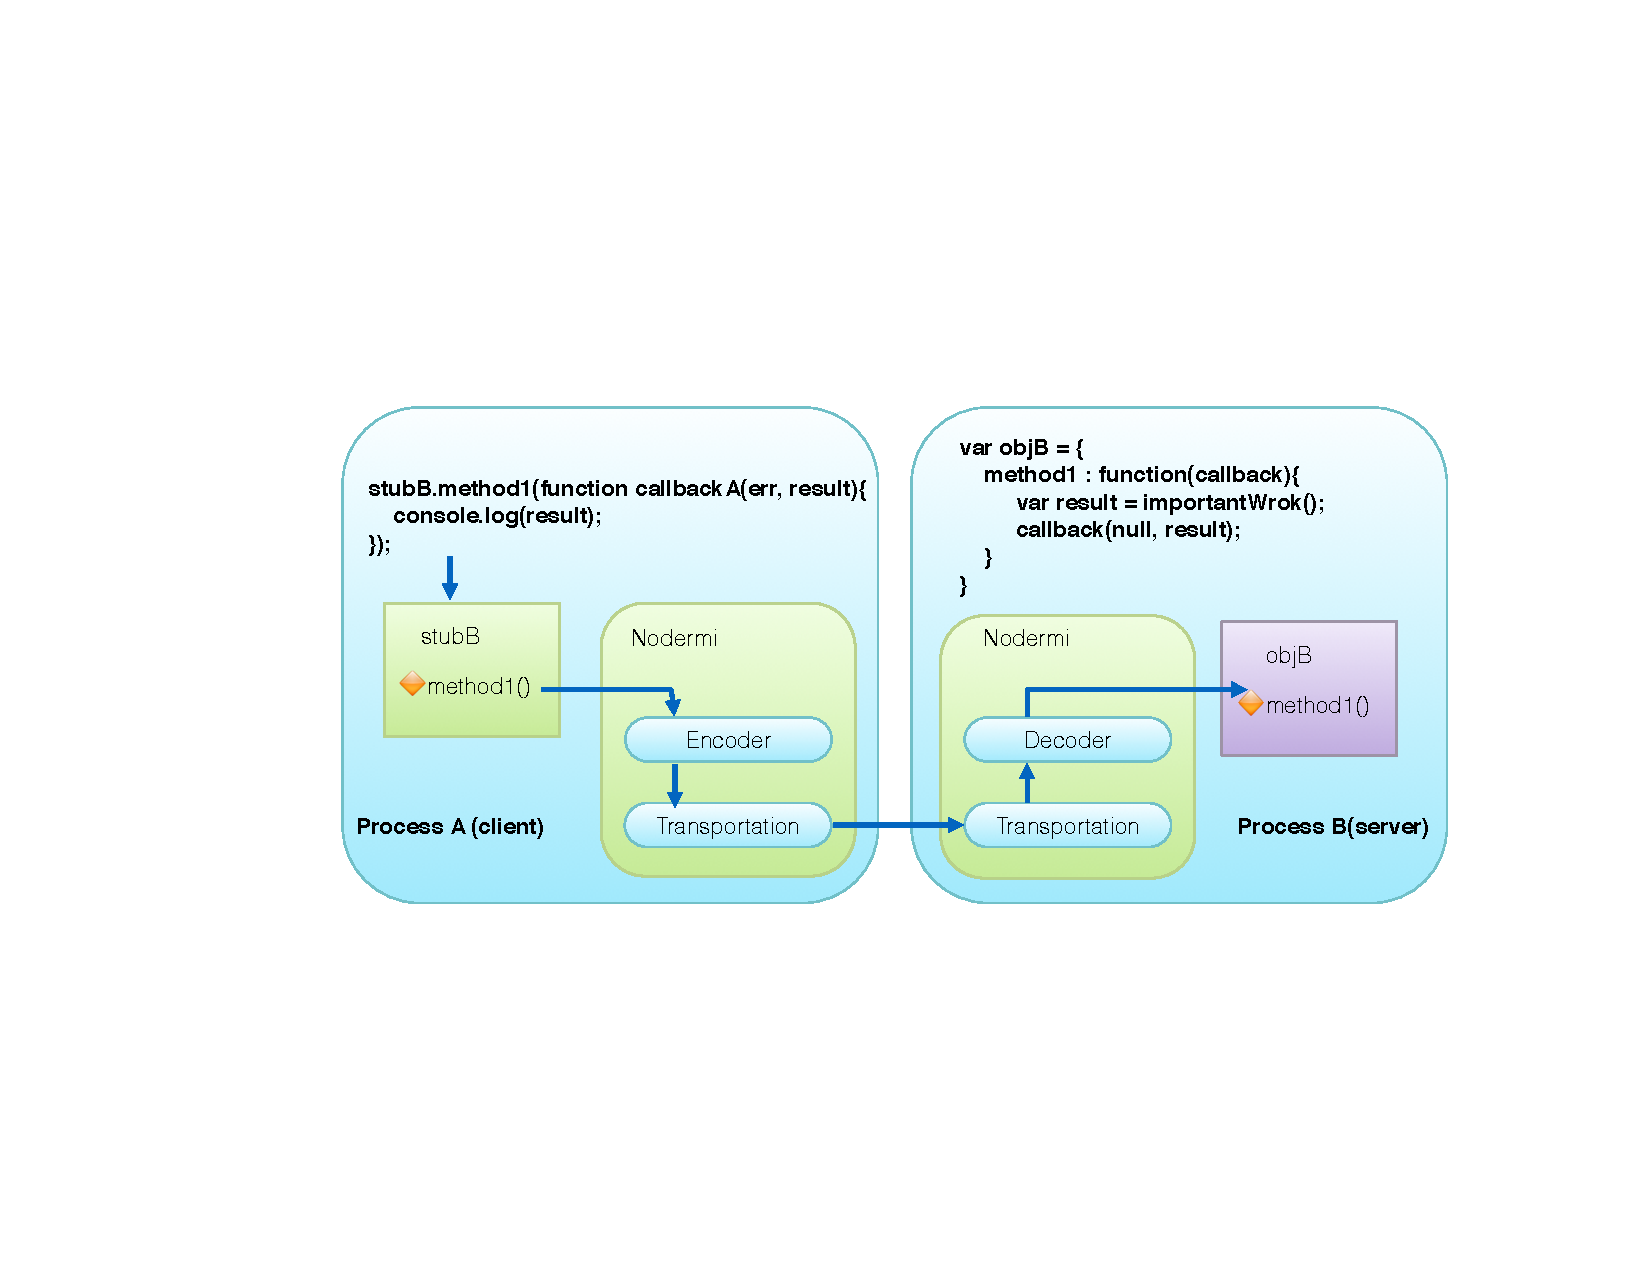
\includegraphics[width=0.8\textwidth]{../figs/nodermi_method_invoke}
    \caption[Remote method invocation via a stub object]{Process A invoke a method of a stub object}
    \label{fig:nodermimethodinvoke}
    \end{figure}
}

% deprecated
\newcommand{\nodermicallbackfig}{
    \begin{figure}[ht]
    \centering
    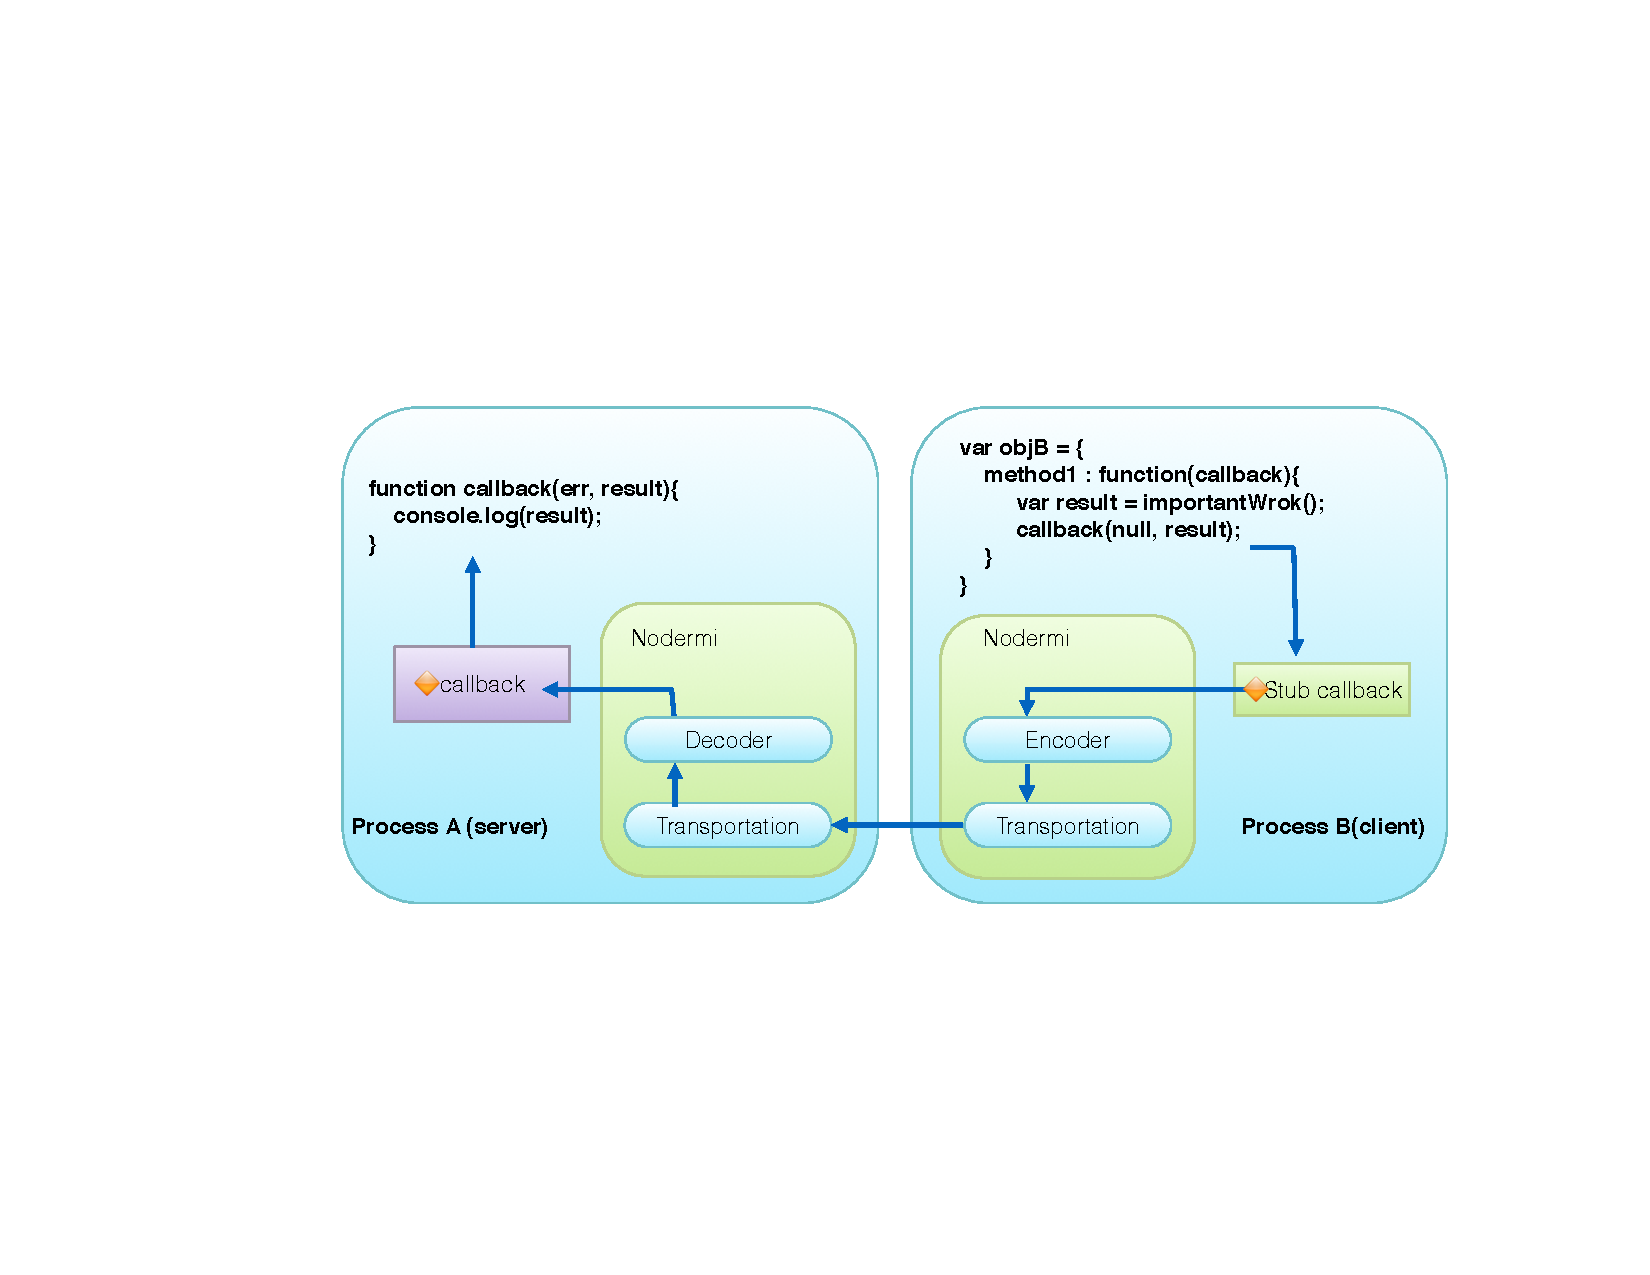
\includegraphics[width=0.8\textwidth]{../figs/nodermi_callback}
    \caption[Remote callback via a stub function]{Process B invoke a callback that itself is a stub}
    \label{fig:nodermicallback}
    \end{figure}
}

\newcommand{\nodermiexamplefig}{
    \begin{figure}[tb]
    \centering
    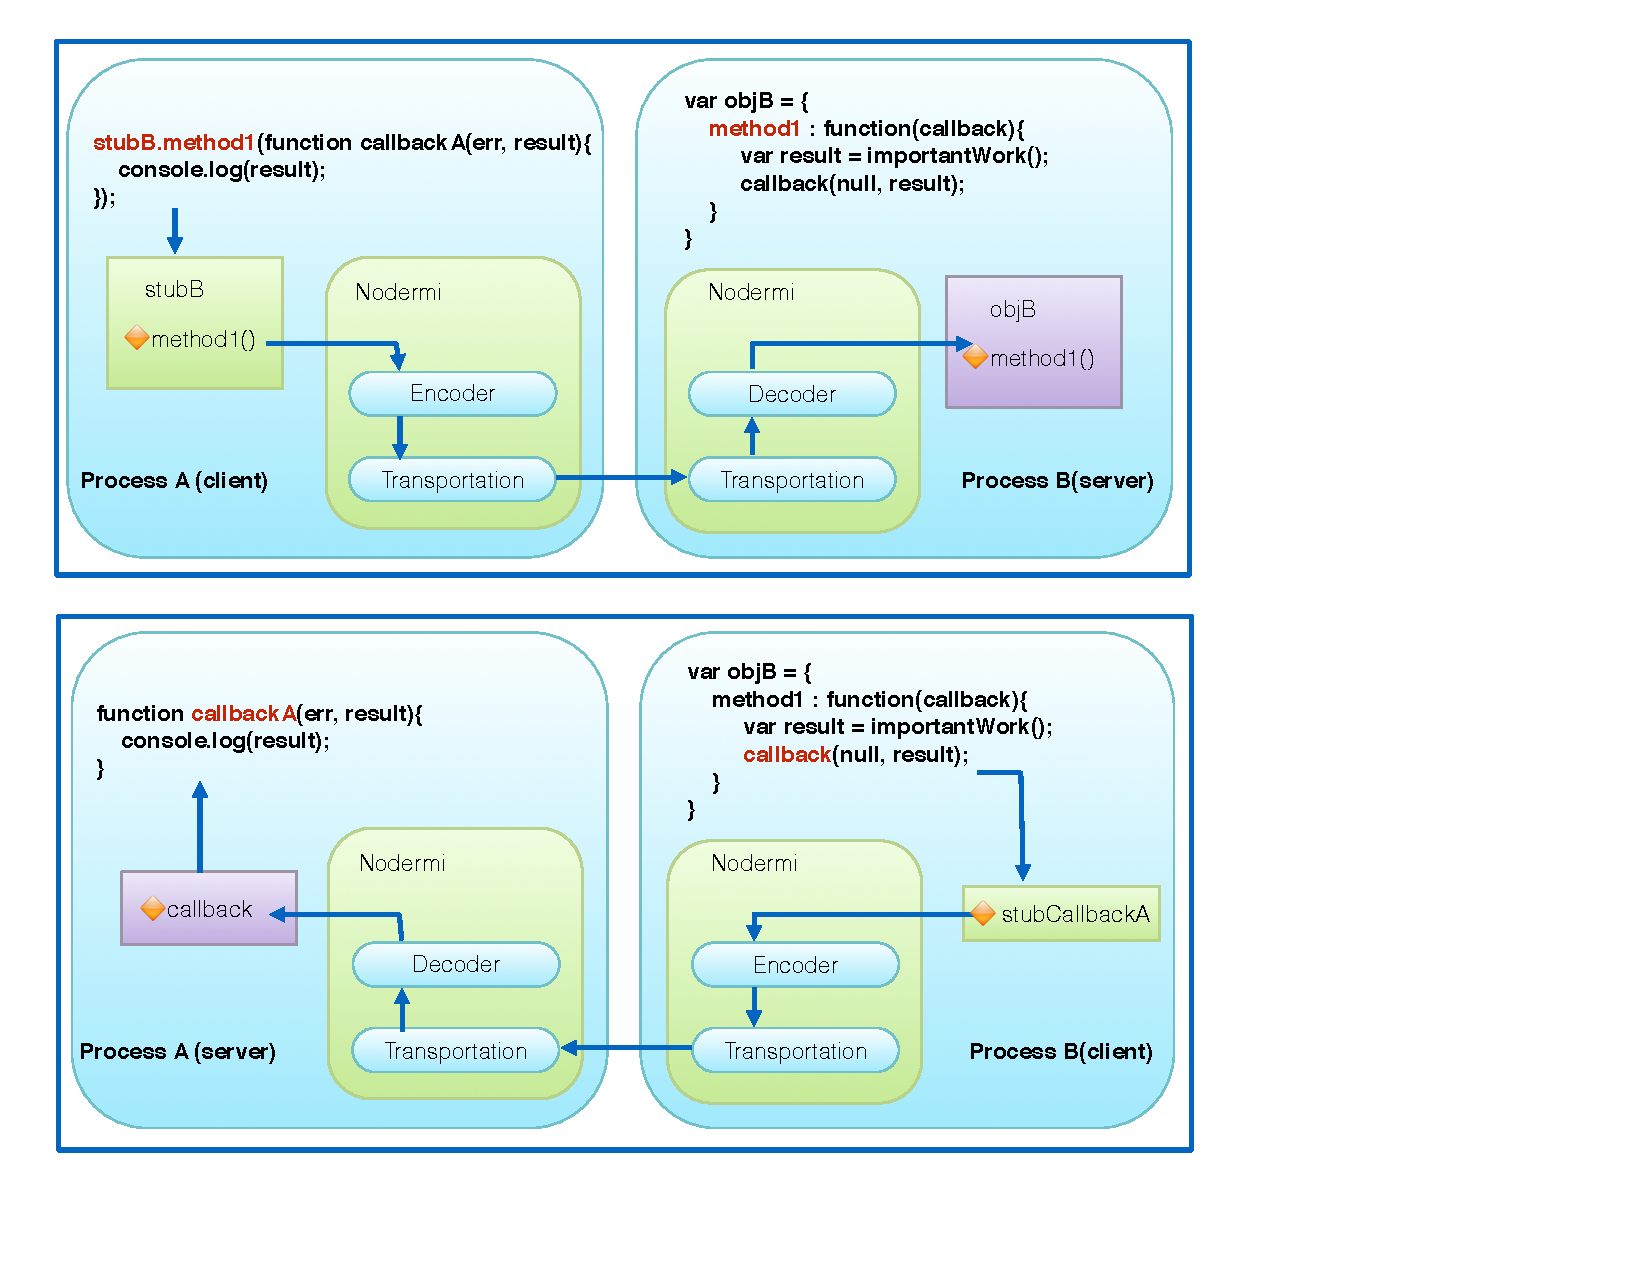
\includegraphics[width=0.8\textwidth]{../figs/nodermi_example}
    \caption{Nodermi remote method invocation example}
    \label{fig:nodermiexample}
    \end{figure}
}

\newcommand{\nodermiobjmapfig}{
    \begin{figure}[tb]
    \centering
    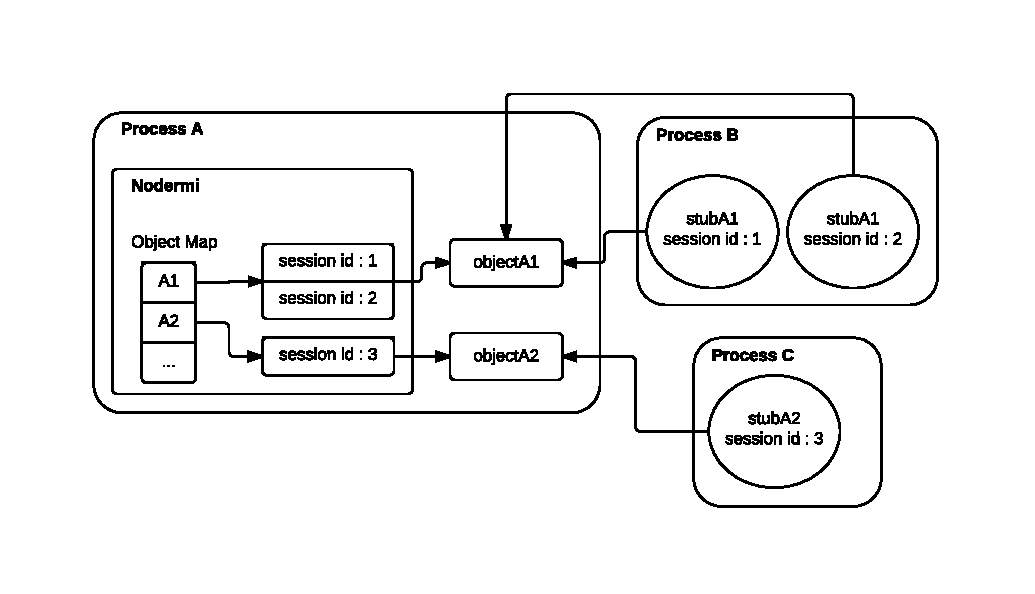
\includegraphics[width=0.8\textwidth]{../figs/nodermi_objectmap}
    \caption[Nodermi memory management]{Nodermi memory management : Nodermi holds 
    strong references to local objects that are remotely referenced in \emph{object map},
    holds weak references to \emph{stub}s in \emph{stub map}.}
    \label{fig:nodermiobjmap}
    \end{figure}
}

%deprecated
\newcommand{\nodermiracefig}{
    \begin{figure}[ht]
    \centering
    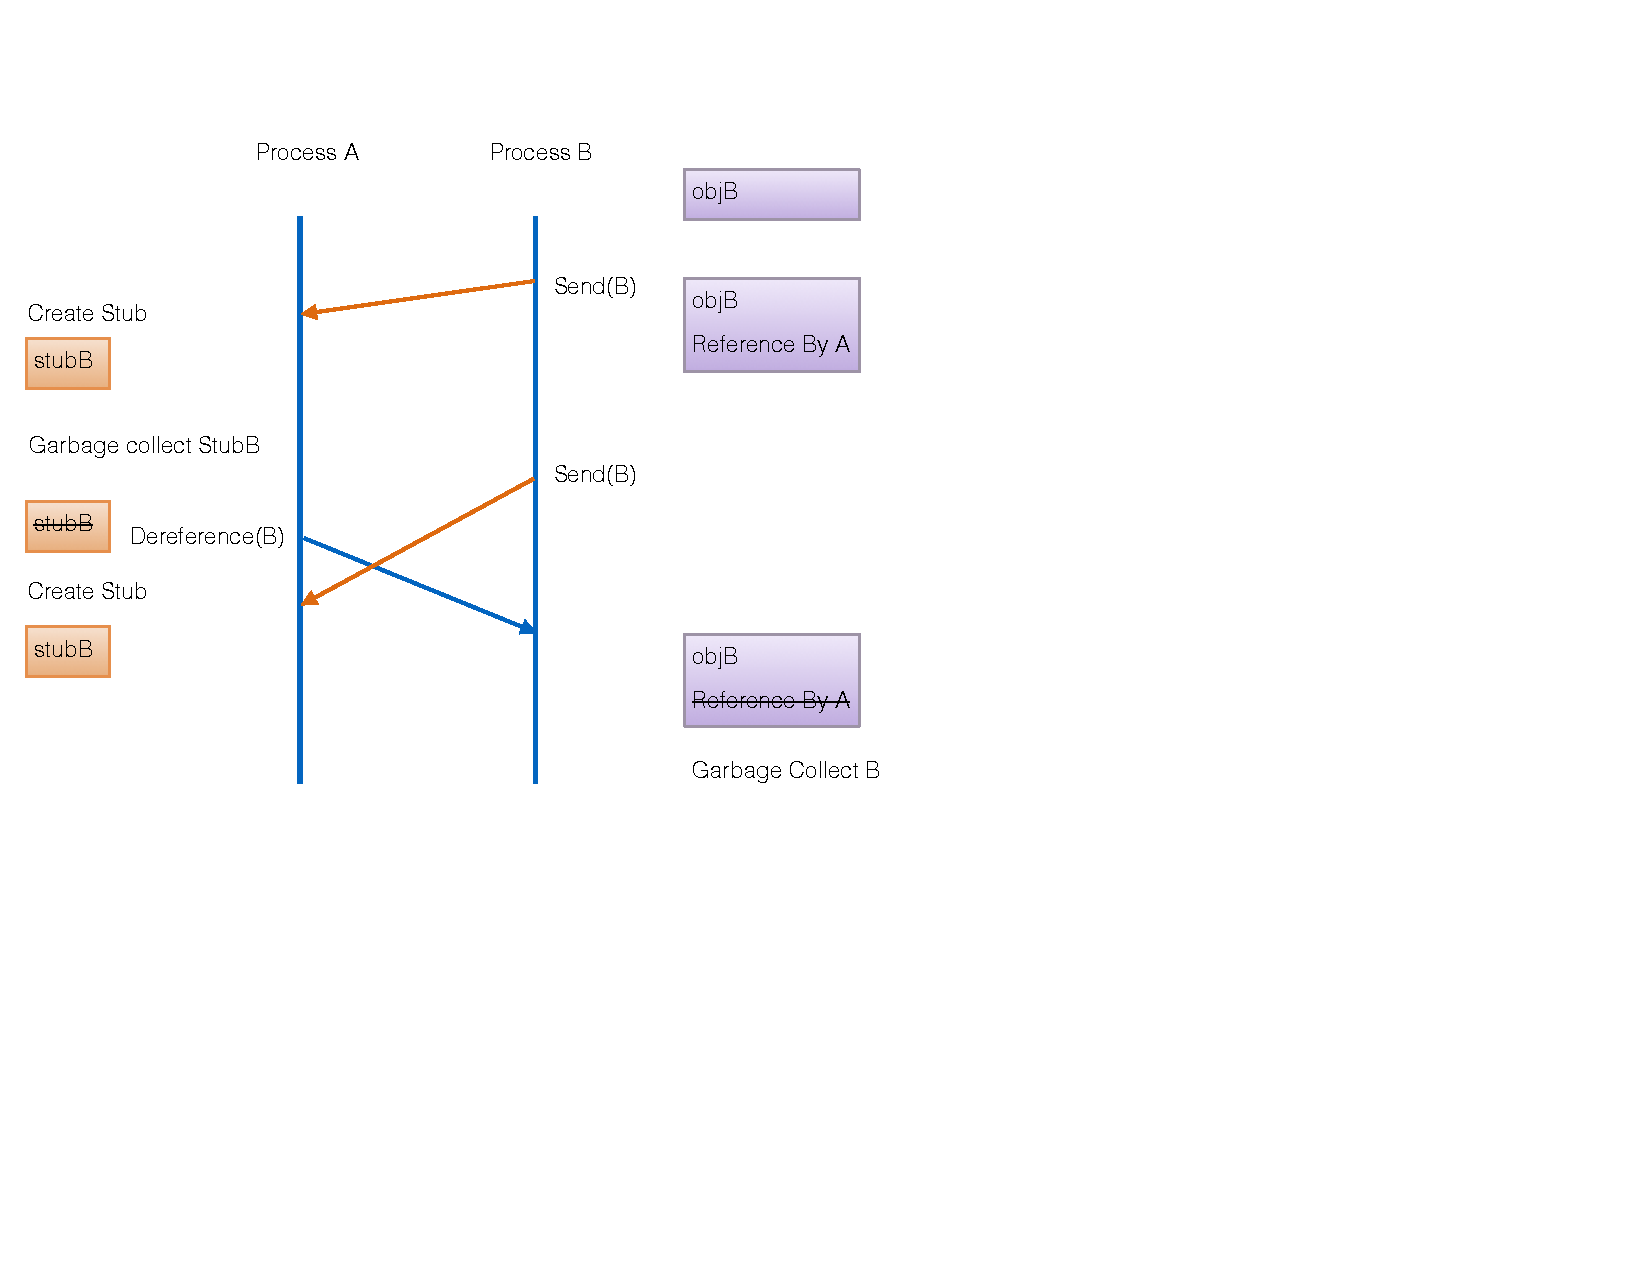
\includegraphics[width=0.8\textwidth]{../figs/nodermi_race}
    \caption[Race condition when dereferencing a remote reference]
    {Race condition when dereferencing a remote reference, \emph{objB} is garbage collected
    when \emph{Process A} still has a stub referencing it.}
    \label{fig:nodermirace}
    \end{figure}
}


\newcommand{\nodermipassbyreffig}{
    \begin{figure}[tb]
    \centering
    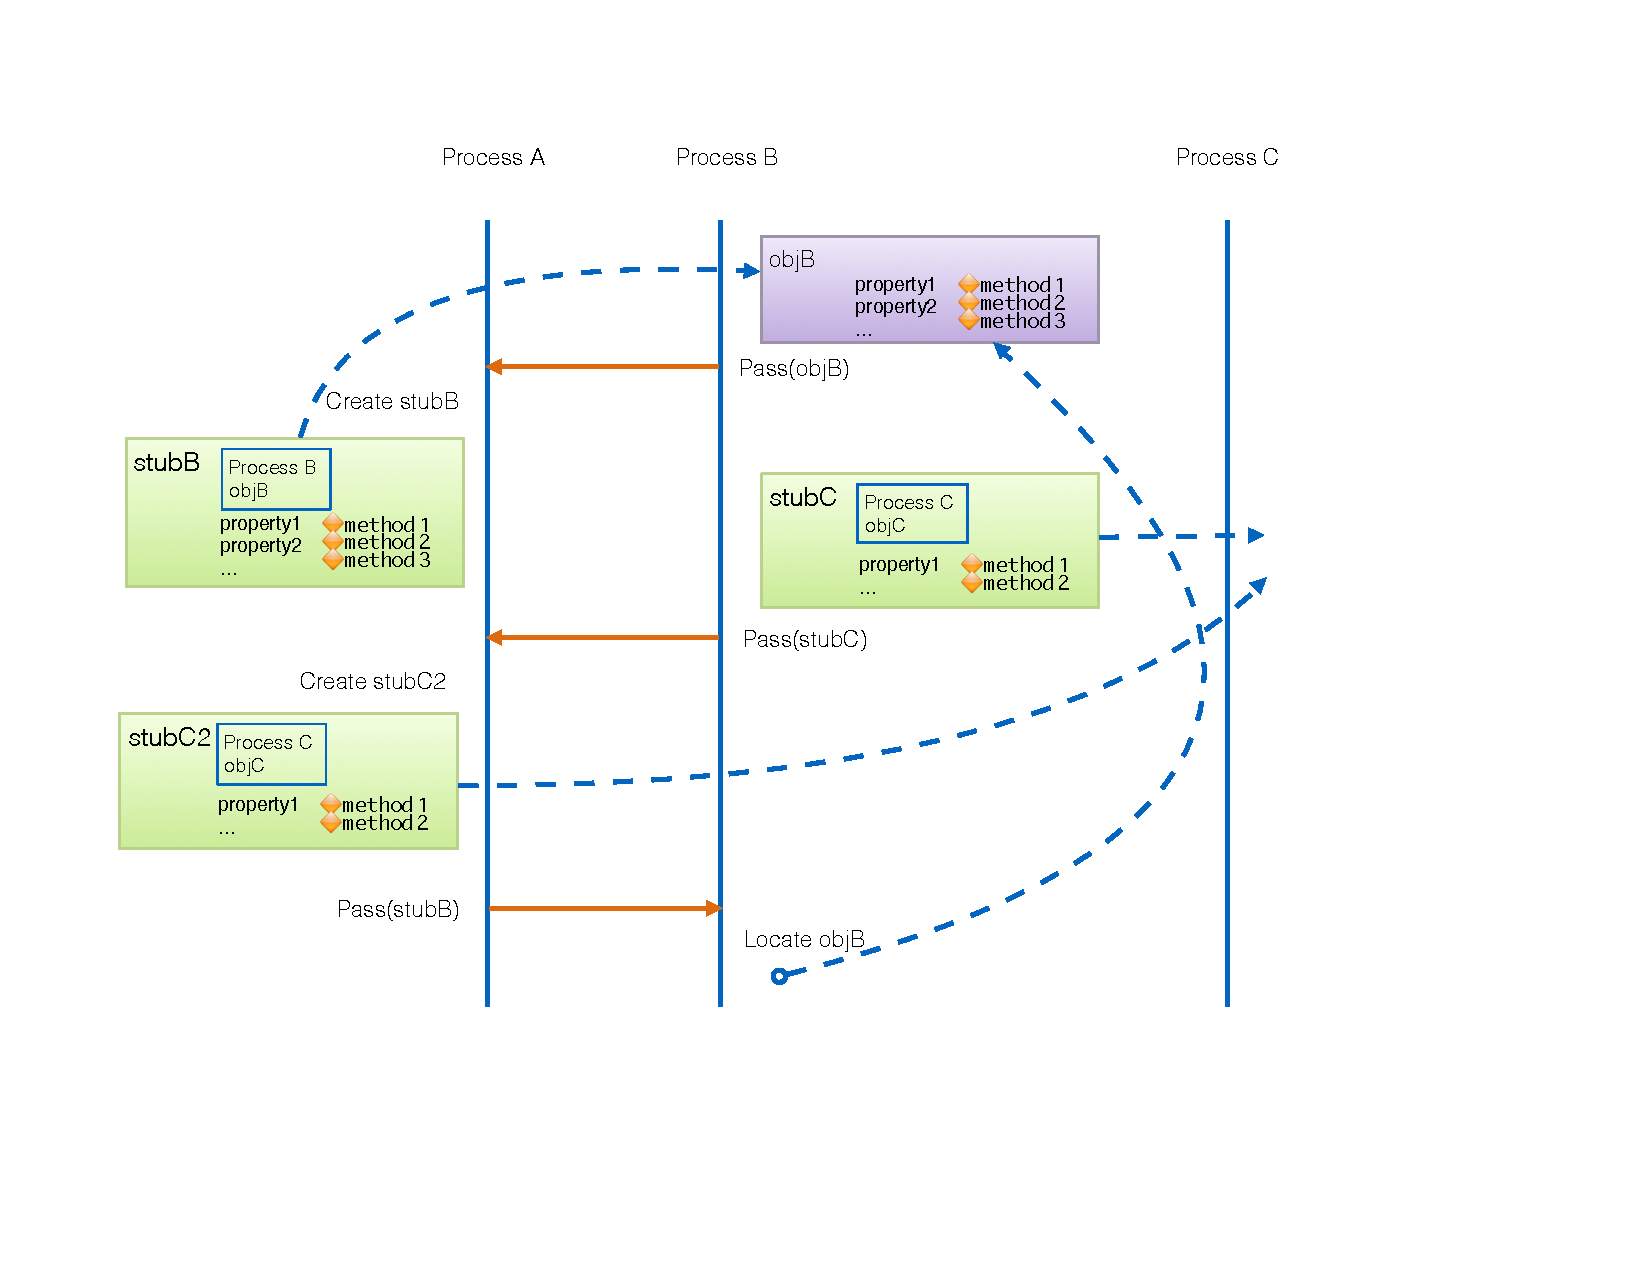
\includegraphics[width=\textwidth]{../figs/nodermi_passbyreference}
    \caption[Nodermi passes arguments by reference]
    {Nodermi passes argument by reference: When passing an argument to a remote
    method call, a remote reference is created for the argument in the server
    process of the remote method. The exception is that 
    when the argument is a stub, nodermi creates
    remote reference for the argument's source object or directly locate
    the source object.}
    \label{fig:nodermipassbyref}
    \end{figure}
}

\newcommand{\nodrmipassbyvalfig}{
    \begin{figure}[tb]
    \centering
    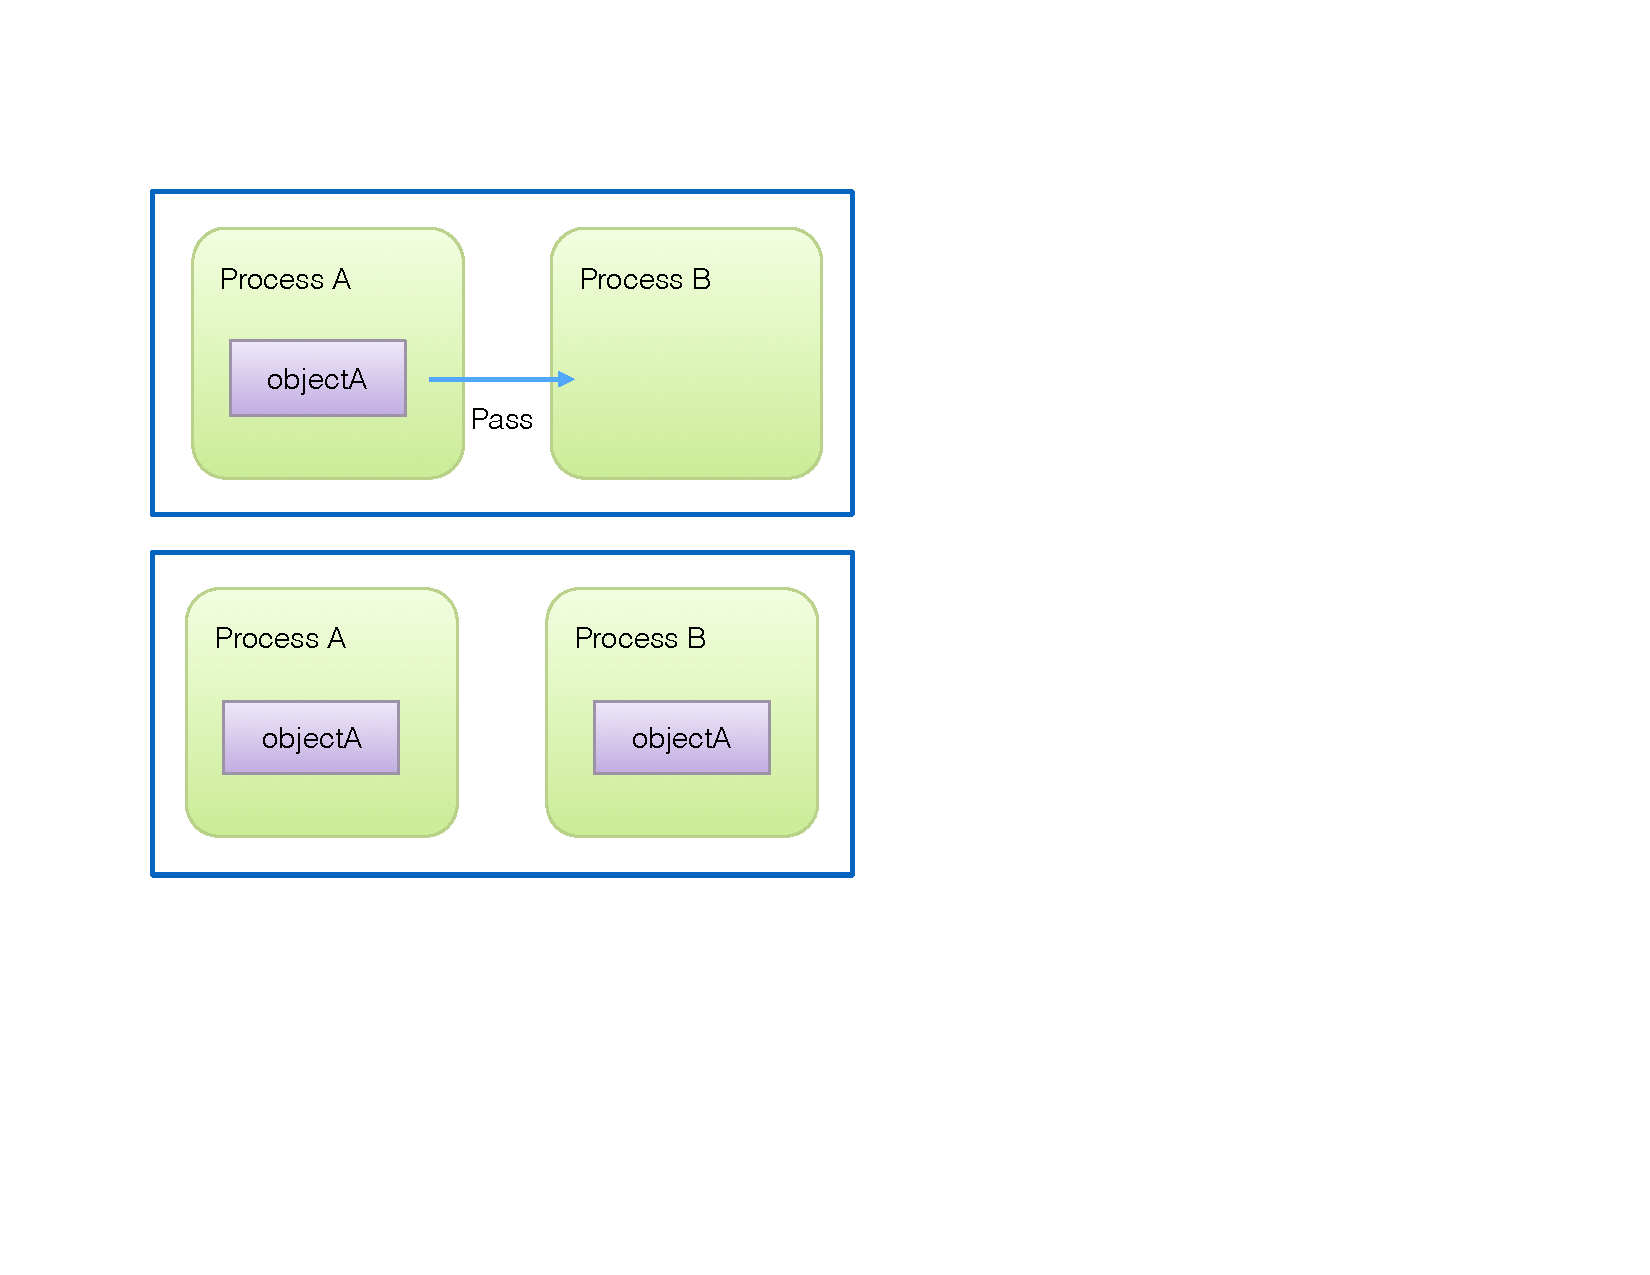
\includegraphics[width=0.8\textwidth]{../figs/nodermi_passbyvalue}
    \caption[Nodermi passes arguments by value]
    {Nodermi passes argument by value: When passing an argument to a remote
    method call and the argument is a simple object with no methods
    , a new copy of the argument is created in the server
    process of the remote method. When the argument is of certain built-in types,
    a new copy is created via constructors, so the new copy has all the methods
    of the original arguments.}
    \label{fig:nodermipassbyval}
    \end{figure}
}

\newcommand{\apiclassfig}{
    \begin{figure}[ht]
    \centering
    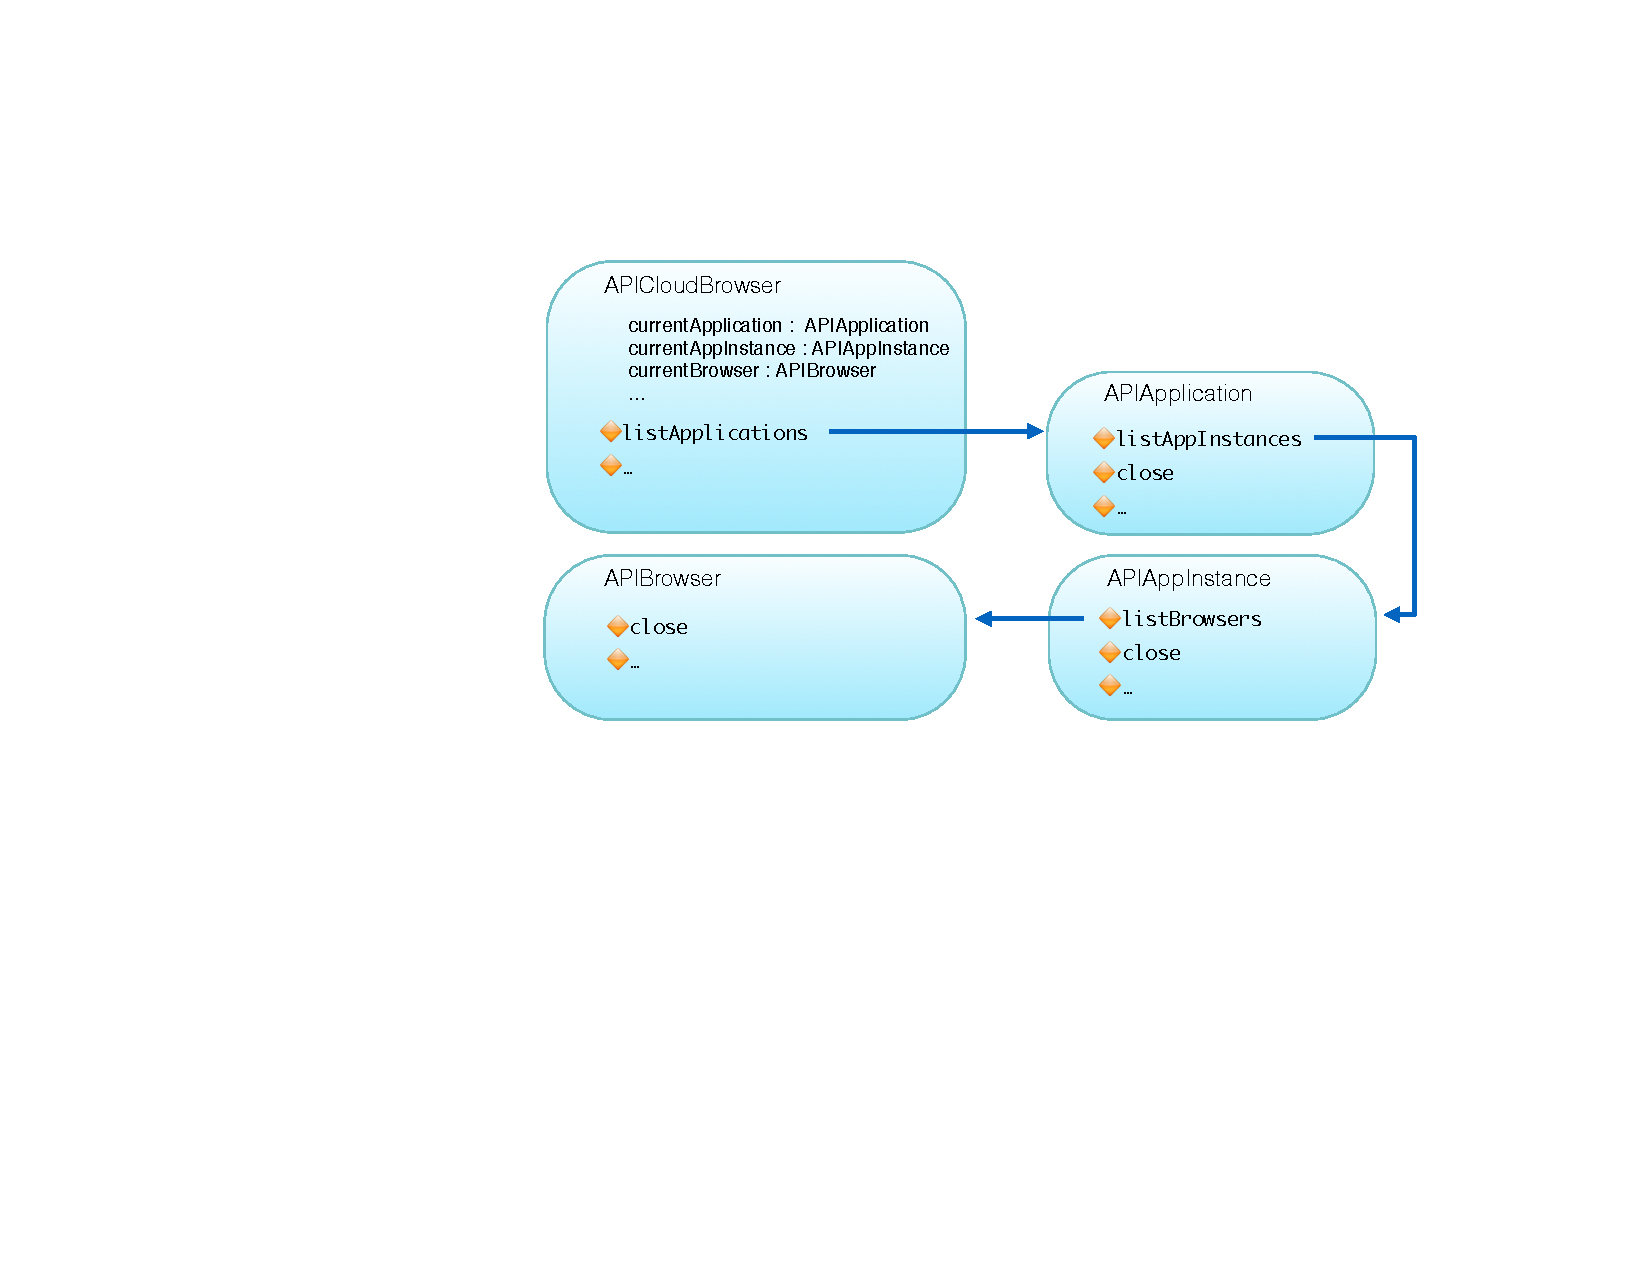
\includegraphics[width=0.8\textwidth]{../figs/api_classes}
    \caption[API class design]{API class design: 
    The arrow points to the method's return value's type.
    For instance,
    The \emph{listApplications} returns
    a list of \emph{APIApplication} objects.
    ``:'' indicates an variable's class, ``currentApplication:APIApplication'' means
     \emph{currentApplication} is a \emph{APIApplication} object.
    }
    \label{fig:apiclass}
    \end{figure}
}


\newcommand{\apireferencefig}{
    \begin{figure}[ht]
    \centering
    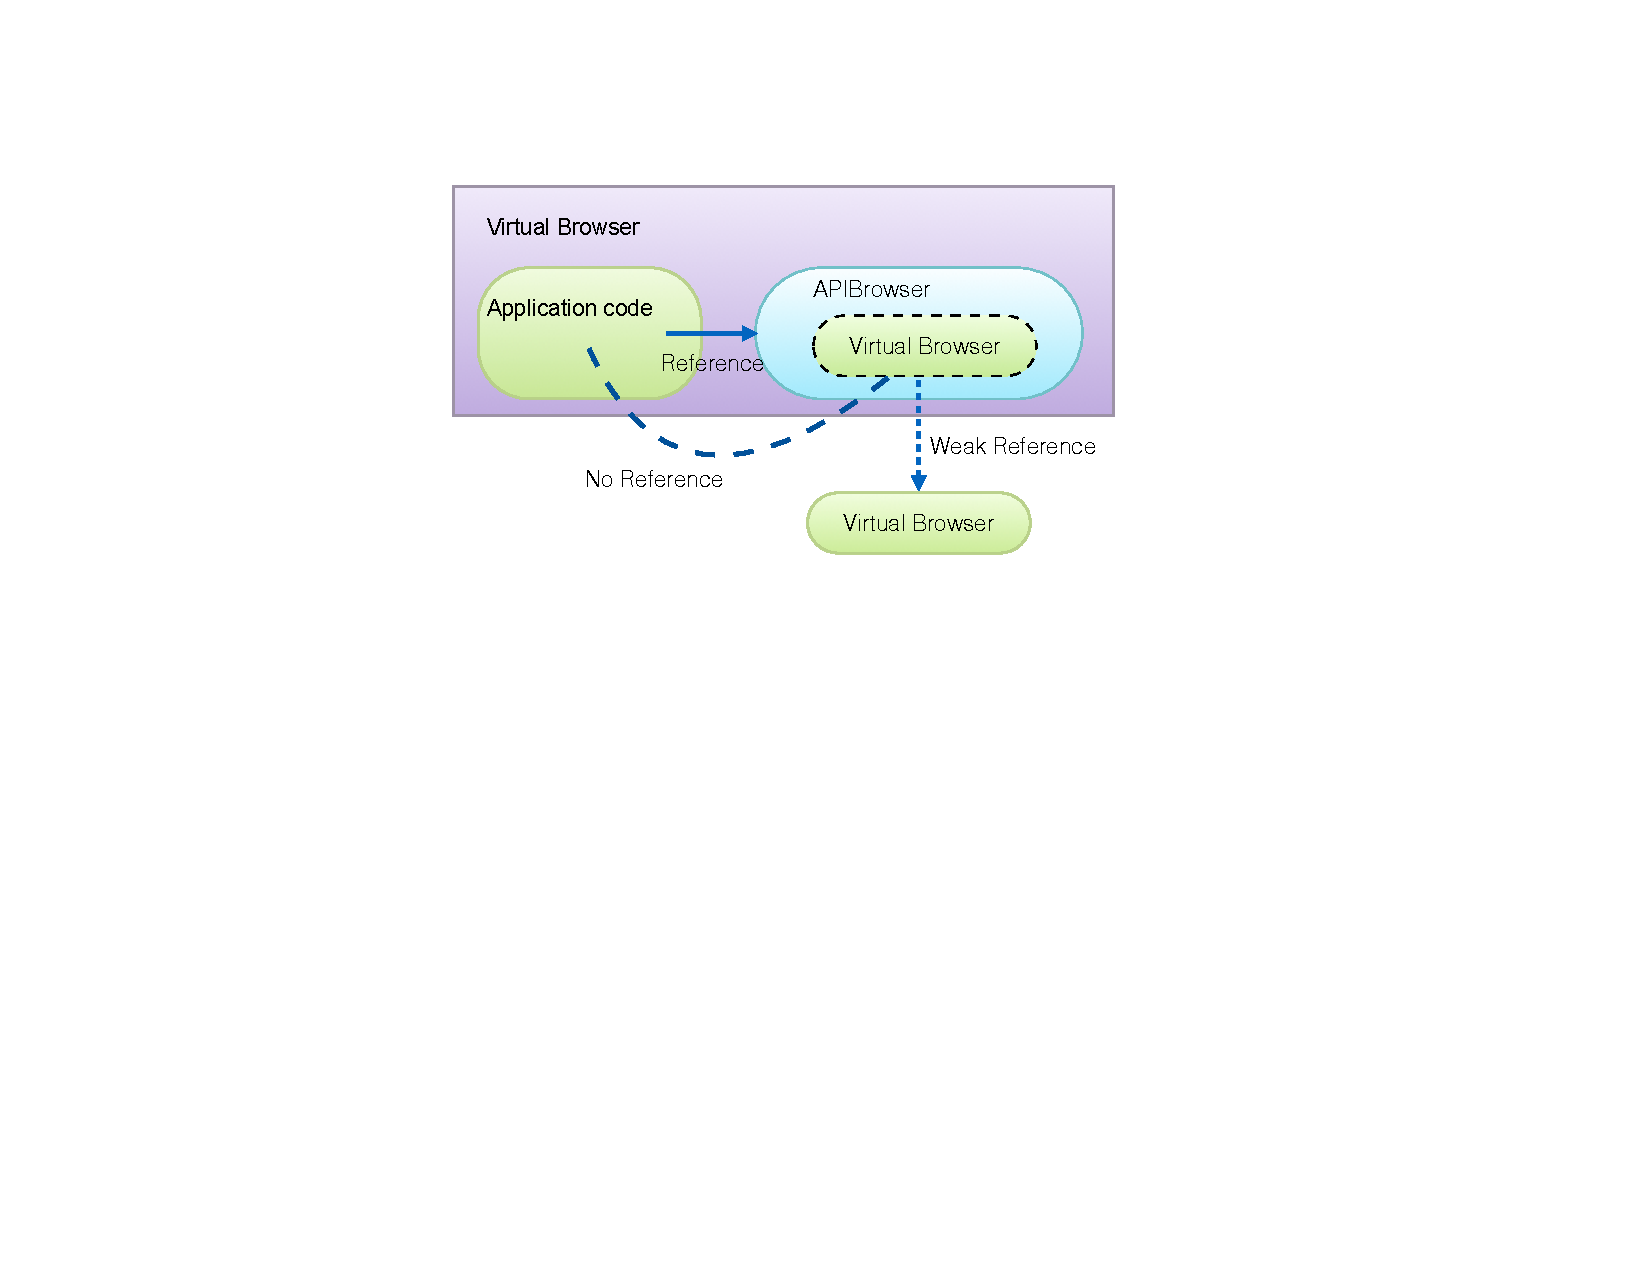
\includegraphics[width=0.6\textwidth]{../figs/api_reference}
    \caption[API object structure]{API object structure : API objects only keep weak reference to internal objects}
    \label{fig:apireference}
    \end{figure}
}

\def\code#1{\texttt{#1}}
\def\nodermi{\texttt{nodermi\xspace}}

\thispagestyle{empty}
\pagenumbering{roman}
\begin{center}

% TITLE
{\Large 
\etdtitle{}
}

\vfill

Xiaozhong Pan

\vfill

Thesis submitted to the Faculty of the \\
Virginia Polytechnic Institute and State University \\
in partial fulfillment of the requirements for the degree of

\vfill

Master of Science \\
in \\
Computer Science and Applications

\vfill

Godmar V. Back, Chair \\
Eli Tilevich\\
Ali R. Butt

\vfill

April 28, 2015 \\
Blacksburg, Virginia

\vfill

Keywords: Web, Javascript, Node.js, Distributed System
\\
Copyright 2015, Xiaozhong Pan

\end{center}

\pagebreak

\thispagestyle{empty}
\begin{center}

{\large \etdtitle{}}

\vfill

Xiaozhong Pan

\vfill

(ABSTRACT)

\vfill

\end{center}

When developing web applications using traditional methods, the developers
need to partition the application logic into a client side and server side,
then implement these two parts separately (probably in two different
programming languages) and write the communication code to synchronize
application state between the two parts. \cb is a server-centric web
framework that eliminates this need of partitioning application entirely. In
\cb, the application code is executed in server side virtual browsers
which also preserves the application's presentation state. The client web
browsers act like rendering devices, they fetch and render representation
states from the virtual browsers. The client-server communication and user
interface rendering is implemented by the framework under the hood. The
applications are developed in a way similar to regular web pages, using no
more than HTML, CSS and \js. Since the user interface state is
preserved server side, the framework also provides a continuous experience for
users who can disconnect from the application at any time and reconnect to
pick up at where they left off.

The original implementation of \cb is single-threaded  and supported
deployment on only one process. We implemented \cbtwo, a multi-process
implementation of \cb. \cbtwo can be deployed on a cluster of servers as well
as a single multi-core server. It distributes the virtual browsers to multiple
processes and  dispatches client requests to the associated virtual browsers.
\cbtwo also refines the \cb application deployment model to make the framework
a PaaS platform. The developers can develop and deploy different types of
applications and the platform will automatically make them scalable.


% To transparently partition the existing CloudBrowser infrastructure
% code across nodes, we designed and implemented an object-oriented RPC
% framework called nodermi for node.js.  Nodermi transparently creates remote
% references during remote method invocations and garbage collects remote
% references when they are not needed. To better understand the limitations of
% the system and assess the feasibility of hosting real-life applications, we
% evaluated the system's performance using different types of applications and
% JavaScript libraries. Our experiments show that CloudBrowser 2.0 scales
% linearly, it can support 2,800 concurrent clients interacting with a non-
% trivial web application using a eight core machine.

% ------------

\vfill

% GRANT INFORMATION

\pagebreak

% Dedication and Acknowledgments are both optional
% \chapter*{Dedication}
% \chapter*{Acknowledgments}
\chapter{Acknowledgments}
\markright{Acknowledgments}

I am very fortunate to have Dr. Godmar Back as my advisor. He is always patient,
even for dumb questions. 
He is strict for every detail, but in the same time gives me enough freedom
to make my own decisions.
He inspires me to be a better engineer and researcher with his great passion for
technology and innovation, and his unparalleled professionalism. 


I would also like to thank Dr. Ali R. Butt and  Dr. Eli Tilevich for serving in my
committee and providing valuable feedbacks.

Finally, I would like to thank my fellow graduate students in computer science department,
it is a honor to spend two years with you wonderful guys. 

\tableofcontents
\pagebreak

\listoffigures
\pagebreak

\listoftables
\pagebreak

\pagenumbering{arabic}
\pagestyle{myheadings}

\section{Introduction}
\label{sec:intro}

% backgroud, motivation, design choices, architecture , experiments(goals, etc.)
Before AJAX~\cite{garrett2005ajax} became pervasive, most web site works like this:
the user sends a request to the web server through submitting a form or clicking a link on a web page,
then the server processes this request and responds a new HTML document.
In this model, the application logic resides mainly on server side, the client side is mostly
plain HTML document.
The problem about this form/link based model is that it is hard
to create responsive and rich user experience because the whole user interface
is wiped out and re-rendered every time user sends a request.

AJAX is an approach that uses javascript to send requests to server
and partially update the HTML document without page refresh.
It is capable of delivering a better performance and native application like user experience.
In this model, developers have to write client javascript code to handle server client communication
and rendering logic. 


\cb{} is a server-centric framework designed to simplify the development of AJAX web applications.
Developer's code is running in a server side virtual browser and the user's browser is just
a dumb display device which synchronizes with the virtual browser.
In \cb{}, developers use nothing but HTML, css and javascript to construct the UI logic just like
any traditional AJAX application.
In the place where traditional AJAX applications call a server side API through HTTP,
developers could call a server side method directly.
The synchronization between the virtual browser and the actual browser is 
handled by the framework under the hood.
\cb{} also naturally preserves UI state upon page refreshes
because all the UI state is kept in the server side.



%Comparing to other server-centric frameworks, 
%\cb{} could reuse most of existing client code because it does not require an extra markup language
%and its sole programming language is javascript.


The original \cb{}'s architecture is restricted to a single process.
It cannot benefit from multiple processors and provides no isolation between virtual browsers.
The stateful nature of \cb{} makes it hard to support multiple process, 
but we think it is a effort worth taking for it would not only boost \cb{}'s capacity
but also shed some light on how to scale nodejs applications in general.





\chapter{Background}
\markright{Background}

This chapter provides background information to understand the concepts
underlying the design of \cbtwo. We assume the reader has basic knowledge of
web-related protocols and languages, including HTTP~\cite{rfc7231},
HTML~\cite{hickson2012html},  DOM~\cite{2000Document},
\js~\cite{ecmascript2011ecmascript} and CSS~\cite{css21}.

\webscaleoutfig{}

\section{Scalable Web Server Architectures}
\label{sec:websys}

\cbtwo aims to provide a scalable platform for web applications.
In this section we introduce some typical methods to design
scalable architectures for web applications.

Web servers provide the infrastructure on which web applications 
are hosted.
Scalability is an important issue for web servers as the number of users
visiting a site can grow significantly~\cite{berners1998world}.
Even without the increase in users,
web applications demand more resources as they become more sophisticated.

Figure~\ref{fig:webscaleout} is a diagram of a typical scalable web server
architecture, which is able to harness resources from a cluster of servers. We
divide the servers in such web systems into two layers. The web layer
processes HTTP requests from users and generates HTTP responses which will be
rendered in the user's browser. The web layer offloads storage and
computational tasks to a storage layer that consists of database servers or
other types of storage servers. The benefit of such layered design is twofold:
it makes the web servers lightweight so they are able to handle more
concurrent  connections; the whole system becomes modular, so that the system
operator can upgrade parts of the system without interfering with other parts.

To balance requests evenly across the web servers, a load balancer component
sits between the clients and the web layer, which dispatches user requests to
web servers and returns the responses from the web servers to users. The use
of a load balancer allows users to access the web server using a single URL
because it hides the distributed architecture from the user. There are many
ways to implement load balancing~\cite{cardellini2002state}. We can use round-
robin DNS~\cite{} to distribute the load to multiple addresses. First, we need
to register a list of IP addresses to the DNS server. The DNS server orders
the registered addresses in round-robin fashion
 and return the ordered
addresses for every DNS query from the user.  The user will use the first
address in the returned list to issue requests. Considering the effect of DNS
caching, some users will send requests to the first address in the registered
list, some users will send requests to the second address in the list, and so
forth. We can expose  all web servers directly to the clients  by registering
all web servers' public IP addresses using round-robin DNS. In this way,
clients directly issue requests to the web servers. However, this solution is
not flexible about adding or removing web servers. To overcome limitations of
DNS based load balancing, people often add a layer of reverse proxies \footnote{A
reverse proxy (such as nginx~\cite{nginx})  forwards user requests to one or
multiple web servers and copies responses from the web servers back to the
users} between the clients and the web servers. We can register the IP
addresses of the reverse proxies to the DNS server. The user requests are
first distributed among the reverse proxies, then  the reverse proxies
distribute user requests across web servers.

From now on, we will only discuss the distribution algorithm without meddling too much
in the implementation details of the load balancer layer.
%
%  REVISE TO HERE
%

% \subsection{Application State Management}% maybe too big a title for a short review...

% We use application state to describe 
% the data web applications need to 
% process user requests and render user interface.
% Based on the design of the web application,
% the application state could comprise data fetched from some permanent
% storage or 
% generated during the execution of the application.
% On the other direction,
% the data in application state could be written back to permanent
% storage or just be kept transiently.
% The application state data that stored permanently could
% endure server restart and be referenced in the future,
% it usually contains data that is costly or impossible to 
% recreate, like user profile, shopping transactions, etc.
% The application state data that is transient 
% usually represents state that is acceptable to be lost
% during server restart or client crash.


% To distinguish individual users, the web application assigns 
% a unique session identifier for each user.
% The session identifier is then attached to every HTTP requests.


\subsection{Session State Management}

The web applications use session state to remember user-related information across HTTP requests
so they can provide user specific service using stateless HTTP protocol.
The session state is store on the server side indexed by session ids.
The web applications assign a unique session id for each user and 
use this session id to retrieve the user's session state for each request.
For the first request, the sever automatically creates a session state for the user.
The applications could store various information in a user's session state
such as user profile, a shopping cart, etc.

Most web frameworks provides two modes to manages session
state~\cite{j2eedoc}~\cite{phpdoc}: a local mode where server side session
data is stored in memory or in file system, a distributed mode where server
side session data is stored in a storage system usually a relational database.

If session state is stored locally, it can be accessed faster, but it is not
accessible from other web server instances.  To overcome this limitation, some
web servers like Tomcat support a session replication
mode~\cite{tomcatcluster} that  synchronizes locally stored session state
across the whole cluster of web servers . Since a web server needs to
broadcast session state changes to all other web servers,  this mode is
expensive when there are many web servers.

Large scale web applications usually adopt distributed mode session.
Besides traditional rational database,
the backend session storage could be implemented by high performance key value
store such as redis or distributed data stores such as memcached, Cassandra, etc.


\subsection{Load Balancing}

In this section we discuss the design choices regarding load balancing and how
its implementation impacts application development.

We use the taxonomy from the survey of Cardellini et
al.~\cite{cardellini2002state} to categorize the load balancer into client-
blind or client-aware based on if the load balancer uses any information from
the client request to perform the dispatch.

A client-blind load balancer does not use information from client when
deciding how to dispatch a request. For example, it could randomly select a
web server from the web layer for each request, or use a round robin
algorithm. In this case, multiple requests from one client could be relayed to
different web servers. In this design, session state cannot be stored locally,
rather it must be accessible  from any server handling the client's request.
For every request, the web server needs to fetch the session state from
session storage and pushes the changes back to session storage if session
state is modified.


A client-aware load balancer dispatches every request from a given client to
the same web server. In this model, the web server can use the local mode
session implementation, which is faster. The web server can also use the
distributed mode to store session data so that the session data could endure
web server restart. Since a given client's requests are dispatched to the same
server, the web server can cache session data to get a better performance.  In
this way,   The web server retrieves session state once for every user and
only communicate with the storage system when session data changes. The
downside for the client-aware load balancer  is that the load balancer needs
to identify each client's assigned server to make the correct routing
decision. For instance, the load balancer needs to examine the HTTP request
header to extract the session identifier and assign web servers based on a
hash of this identifier.

Because different request can impose different load on a web server, the
simple implementations mentioned above can cause uneven load distribution
among web servers. Especially for modern web applications with long
connections, the time a connection keeps open can vary from milliseconds to
hours. A naive load balancer can keep distributing requests to an already busy
server when there are servers idle in the cluster. The load balancer can also
be server-aware such that  it  takes servers' load information into
consideration when making dispatching decisions. Because client-aware load
balancing has the restriction of keeping requests from a given user to the
same server, server-aware client-aware load balancing is more complex than
server-aware client-blindness load balancing.
 
% Another aspect that needs to be consider to design a scalable web system
% is the servers' load.
% The servers' load could be drastically uneven if the load balancer
% does not take the servers' state into the distribution process.

% Current web frameworks usually only deals with the Client Layer and the Web Layer,
% the web application developer should take the distribution policy of the load balancer
% into consideration when designing web applications,
% and they would need to configure or implement the load balancer to support
% the needs of the application.


% Current web frameworks do not have clear construct to define application state.
% One option for the developer is to rely on session objects provided by frameworks.
% The application developer needs to configure the persistence  of session objects
% and make sure the configuration works with the load distribution scheme.
% For example, in J2EE the session objects could be configured to be managed in memory or
% high available database~\cite{j2eedoc};
% in PHP developers could specify a session save handler to store session objects
% in database~\cite{phpdoc}.
% By default, these frameworks store session objects in memory or in local file system.
% If the developer adopts a client-blind load balancer,
% he needs to configure the session objects to use database or other
% synchronization mechanism to make sure the application state could be fetched on every server.
% Another option is to implement his own way of handling application state.
% Regardless of the choices of managing application state,
% the developer needs take the distribution policy of the load balancer
% into consideration when designing web applications,
% and in the other direction,
% the developer needs to find the right load balancer to support his application.






\section{\nodejs}

\cb is written in \nodejs. \nodejs~\cite{tilkov2010node} is a standalone \js
runtime built on Google Chrome's V8~\cite{v8} \js engine that allows \js code
to be executed without a web browser.  \nodejs comes with a standard library
that provides API for file system access, network IO, binary data
manipulation, etc. It enables developers write server side network
applications using \js.  \nodejs is appealing for building high performance
scalable web applications because it adopts a non-blocking event driven IO
model which is capable  to handle a large number of concurrent connections
using a single thread.

\nodejs has a thriving community with a variety of third party packages.
We have relied on a lot of packages in \cb to implement complex tasks like
server side DOM or provide small useful functions like formating a date object.

Another reason we chose \nodejs is that we can write  \cb and the applications
using the same language, there is no language crossing cost.

In this section we will discuss the \nodejs's non-blocking IO model and some
important third party packages we used.

 % it is not parallel with the next section
\subsection{Non-blocking IO}

\begin{listing}[ht,width=\columnwidth]
\begin{minted}[
frame=lines,
fontsize=\scriptsize,
linenos
]
{javascript}
var fs = require('fs');
fs.readFile('/etc/passwd', function (err, data) {
  if (err) throw err;
  console.log(data);
});
console.log("Reading file");
\end{minted}
\caption{Reading file and printing the content on console using \nodejs.}
\label{code:nodefile}
\end{listing}

Listing~\ref{code:nodefile} shows the non-block IO concept in \nodejs. Because
the IO API such as \code{readFile} does not block, line 6 will be executed
before line 3. To wait for the IO operation completes, the developer needs to
register a callback function in the IO method  to be fired asynchronously. In
this example, the callback function is placed on the event loop after the
file's content is read, then the runtime will dequeue this callback sometime
in the future and execute it. Unlike languages that support multiple threads
where code can be executed concurrently, \js runtime has only one execution
thread and it does not block. In this way,   thus the programmers do not need
to use mutual exclusion mechanisms like Locks. The drawbacks of this model is
that the programmers need to manually maintain the application context in the
callbacks  and  it is hard to reasoning the execution order of the code.
Listing~\ref{code:nodefile2} shows the necessity for programmers maintain the
application context in callback. Without keeping the current \code{fileName}
in closure using \code{createReadFileCallback}, line 18 will always print the
last \code{fileName} while line 6 will print the correct \code{fileName}.
There is also no guarantee that the callbacks will be called in the same order
they are registered because the events for these callbacks can happen in any
order. For instance, in Listing~\ref{code:nodefile2} line 6 the files can be
print in any order although their callbacks are registered in a fixed order.
It is also possible that a function that accepts a callback function executes
the  callback synchronously,  thus making the reasoning of the execution order
more difficult.


\begin{listing}[htb,width=0.8\columnwidth]
\begin{minted}[
frame=lines,
fontsize=\scriptsize,
linenos
]
{javascript}
var fs = require('fs');
var files = ['/etc/passwd', '/etc/hosts'];
var createReadFileCallback = function(fileName){
    return function(err, data){
        if (err) throw err;
        console.log("content of " + fileName + " is "+ data);          
    }
};
for (var i = 0; i < files.length; i++) {
    var fileName = files[i];
    fs.readFile(fileName, createReadFileCallback(fileName));
};
for (var i = 0; i < files.length; i++) {
    var fileName = files[i];
    fs.readFile(fileName, function(err, data){
        if (err) throw err;
        // this will always print "read /etc/hosts"
        console.log("read " + fileName);          
    });
}
\end{minted}
\caption{Reading 2 files in a loop using \nodejs.}
\label{code:nodefile2}
\end{listing}



\subsection{Important \nodejs Packages}

\subsubsection{Node-http-proxy}

Node-http-proxy~\cite{nodeproxy} is a \nodejs package for developing HTTP proxies.
It provides programming interface to relay a HTTP request to another server and
automatically copy the response from that server to the original requester.
It also supports WebSocket~\cite{rfc6455} protocol.
WebSocket is a TCP-based protocol which provides bidirectional full-duplex communication
mechanism for web browsers.
Using WebSocket, the server could send content to the client without requested
by the client.
Because WebSocket sends messages while keep the connection open,
it is cost efficient comparing to using HTTP requests.
We use WebSocket to implement DOM synchronization between client and server so
the server could push DOM changes to clients.
In node-http-proxy,
the programmer needs only to provide the destination server on the hand shake
request and all the subsequent WebSocket messages will
be transparently proxyed to the destination server.

\subsubsection{Jsdom}

Jsdom~\cite{JSDOM} is a \nodejs package which provides a \js implementation of 
DOM API. We use jsdom to implement server side DOM tree.
Jsdom works like a web browser except it does not render the DOM tree:
it reads HTML documents to build the initial DOM tree,
it also executes \js files specified in script tags.
It is possible to create multiple jsdom instances in a same process,
each of these jsdom instance will have its own DOM tree and
script execution environment,
the scripts in each jsdom instance will have its own isolated view of global variables.
In our model, each virtual browser has one jsdom instance and
forwards client events to the jsdom DOM tree.
We also patched jsdom to get notifications for DOM updates.


\section{\cb}

\architectureoverview{}

In this section we sketch the implementation of
the original single process version \cb{}~\cite{mcdaniel2012cloudbrowser}.
Figure \ref{fig:cb1arch} shows the relationship
between the client engine running in the user's browser and the virtual browser
running server side.  When the user visits the application, the client engine
code is downloaded and restores the current view of the application by
copying the current state of the server document.  Subsequently, user input
is captured, forwarded to the server engine inside the virtual browser,
which then dispatches events to the document.  All application logic runs
in the global scope associated with the virtual browser's window object.
Since the server environment faithfully mimics a real browser, libraries
such as AngularJS~\cite{hevery2009angular} can be used unchanged to implement the user interface.
Client and server communicate through a lightweight RPC protocol that is
layered on top of a bidirectional WebSocket communication.
Stylesheets, images, etc. are provided to the client through a resource
proxy.

\subsection{Deployment Model}
\label{sec:deploymodel}
\appbundlefig{}
As shown in Figure~\ref{fig:appbundle}, 
a \cb application bundle is a directory
contains descriptor files, an entry point HTML file,
\js files and resources files like CSS files, images, etc.
The descriptor files specify the application's name, owner, mount point, and
other application's configuration.
Mount point is the URL path to the application, for example,
if a \cb is deployed at \url{example.com} and an application's mount point is
\emph{chat}, the user could access the application at \url{http://example.com/chat}.
The \js files include libraries like AngularJS or JQuery
, the application code and an optional application instance(explained 
in Section~\ref{sec:appins}) definition.
Like in regular browser, the entry point HTML should have script tags
specifying the \js files the developer wants to be executed in virtual browsers.

The developer could put the application bundle in \cb's application 
directory or upload the bundle using \cb's administrator application.
Multiple applications could be deployed simultaneously.

\apphierarchyfig{}

As emphasized in Figure~\ref{fig:appidhierarchy},
an application could create multiple application instances,
each application instance could create multiple virtual browsers,
a virtual browser could be simultaneously accessed by multiple clients.
% For example, in our chat room example application, multiple clients
% can join one chat room and each client get his own view of the
% chat room.
% In our model, the chat room concept is represented by application instance,
% the user's view of chat rooms are represented by virtual browsers.
% When a user request the chat room application's URL,
% he is redirected to a page that lists all the chat rooms(in essential application instances) 
% he joined.
% From there, the user could manage his application instances.
% He could create a new application instance(chat room) and share the application
% instance's URL to let others join in.
% When a user joined a chat room,
% a virtual browser is created for him so he could interact with the application.
% A virtual browser could also be accessed by multiple clients,
% the DOM updates from the virtual browser will be broadcast to all connecting
% clients to provide a co-browsing experience.



\subsection{Application Instance}
\label{sec:appins}
\appinstancefig{}


Application instance allows multiple virtual browsers to share data structure.
As in Figure~\ref{fig:appinstance} shows, 
every virtual browser is created inside an application instance
and virtual browsers inside an application instance share application instance object.
The application instance itself
consists metadata about the application instance object
 such as ownership and access permissions.
The application instance object is defined
the application instance definition file 
in the application bundle (see Figure~\ref{fig:appbundle}).
When a virtual browser is created in the application instance,
the application instance object is injected into that virtual browser
and the application code could reference it directly.

\chatappfig{}

As an example, consider a scenario for a Chat application developed using AngularJS,
depicted in Figure~\ref{fig:chatapp}.
A system administrator of a \cb deployment would install the application, which give users the
ability to create application instances. To start a chat site, a user would create
an application instance and share its URL with chat participants.  As the participants join
the chat site, a virtual browser is created on demand for each participant, which is connected
to the application instance (the users can bookmark their virtual browser's URL to later return.)
The shared application instance data in such an application
consist of the chatroom(s), users and their associated messages.  The advantage of this design
is that AngularJS's dirty-checking mechanism will reflect updates to the shared instance data
in each virtual browsers' document automatically, thus ensuring that new message are broadcast
to each.

\subsection{Authentication}

When an application is enabled with authentication, the system will redirect
the user's request to a login page if it detects the user has not logged in
that application. The login page itself is implemented by creating a virtual
browser in the system login application. The login page provides two
authentication options: a local authentication option where the user's
credentials are stored in MongoDB; an OAuth~\cite{hardt2012oauth} option which
authenticate user via Google's openID. The user could submit his email address
and password directly in the login page  for local authentication option. Then
the system will find the matching record in the account table.   For the OAuth
option, the user clicks a \emph{Login with Google Account} link  to land on a
Goolge account authorization page. After the user authorizes \cb{} to access
his Goolge account information, Goolge will request \cb{}'s authentication
callback URL and \cb{} will get the user's email address.

After the user logs in using either mode, the system adds an entry of the
user's email address and the application's mount point in the user's session
(stored in MongoDB as well). That entry indicates the user has logged in the
application. Then the login page virtual browser is closed and the user is
redirected to  the URL he originally requested. The subsequent requests from
the user will pass the authentication check until the session expires or the
user logs out the application.


\subsection{Application Instantiation Strategy}
\label{sec:appinstantiation}

The application instantiation strategy specifies
how the application instance and virtual browsers are instantiated.

Application programmers can create CloudBrowser applications in the same way in which
they create the client-side portion of a client-centric application, using low or high level
JavaScript libraries such as jQuery~\cite{jquery} or AngularJS.  
A descriptor in the application's manifest describes 
their application's instantiation strategy.
The supported strategies include

\begin{description}

\item[singleAppInstance] The application supports only one instance and single virtual browser.
    All connected clients will share a single server-side document in this singleton - this can be
    used for applications that display data, such as a weather application. These applications will not
    typically react to user input and users do not need to be authenticated.

\item[singleUserInstance]  This application requires authentication to establish a
    user identity, which we provide through a local database as well as through external OpenID
    authentication.   In this mode, users may not create more than one virtual browser per
    application instance.  When a user accesses the application instance's URL, they will either
    be forwarded to their virtual browser or a virtual browser will be instantiated for them.

\item[multiInstance]
    Allows users to have multiple, separate virtual browsers connected to an application
    instance. For instance, a user may have to be in two separate chatrooms offered by one chat site.
    In those cases, the user has the largest flexibility, but will need to manage whether
    to join an existing virtual browser or create a new one when they visit the application instance
    - similar to the choice a user may have when deciding whether to navigate to a new site in
    an existing browser tab or open a new one.

\end{description}

Except for multiInstance applications, the existence of virtual browsers is not exposed to
end users that merely join existing application instances.


% The hierarchy that results from applications, application instances, and virtual browsers is
% depicted in Figure~\ref{fig:appidhierarchy}.  This figure shows the general case in which an
% application might allow multiple instances, and in which each user can create multiple virtual
% browsers.



\chapter{Nodermi: A Remote Procedure Call Framework for \nodejs{}}
\label{ch:rmi}
\markright{nodermi}
In the single process version of \cb,
everything lives in the same address space,
which allows application code to invoke system components' functionality.
As \cbtwo divides \cb into multiple processes,
some of those local method invocations need to be replaced by
inter-process communication,
because as the framework spreads its state
and responsibility to multiple processes,
an operation initiated in one process
could require access to state located in another process.
For example,
in the single process version,
closing a virtual browser
is implemented by invoking the \code{close} method of the virtual browser
object.
If the virtual browser is in another process, closing it requires that a request be sent to that process.
We could have introduced new objects and methods to send specific messages,
but this approach is undesirable for the following reasons.
First, there are many call sites that would need to be changed.
Second, we would also have to design message formats for many different methods and
write handler code to parse and process each of these messages.
Third, since our codebase is continuously evolving, any changes to existing methods
would require modifications to the message communication layer.

To avoid having to manually create and maintain messaging code for each
method, we developed nodermi~\cite{nodermi}, an object-oriented
remote procedure call (RPC) framework for \nodejs{}.
% Nodermi hides the complexity of inter-process communication details from
% upper layer code and is adaptive to code changes.

Before we discuss the implementation of nodermi,
we first introduce some terms for nodermi and
RPC systems in general.
We use the term \emph{local object}
to refer to objects that are allocated by the calling process.
We use the term \emph{remote object} to represent objects that are
located in processes other than the calling process.
We use \emph{stub} or \emph{remote reference} to refer to special objects created
by nodermi that represents \emph{remote object}s in the calling process
(we can think of \emph{stub}s as proxies to remote objects).
We say an object is \emph{remotely referenced} from a process
if there are \emph{stub}s representing it.
Each \emph{stub} represents one \emph{remote object} and
it has methods that mirror the \emph{remote object}'s methods.
From the programmer's perspective,
\emph{stub}s appear like ordinary local objects.
When calling a \emph{stub}'s method, the underlying
RPC framework code sends messages to the \emph{remote object}'s process
to invoke the corresponding method there.
For a given stub,
the object it represents is called its \emph{source object},
the process that creates the \emph{source object}
is referred to as the \emph{host} of the stub.
The \emph{host} process takes on the role of a \emph{server},
whereas the process that holds a \emph{stub} to the object act as a \emph{client}.
In \js{}, since functions are first class citizens, it is possible
to pass a function as an argument or return a function as a result.
Nodermi treats functions and objects alike so that functions can also be
referred to remotely.

% -------- TODO mention the example

\section{Semantics}
\label{sec:semantics}

\nodermiexamplefig{}

\paragraph{Synchronous Methods}
Unlike RPC frameworks in which a calling process blocks during the
completion of the remote method~\cite{birrell1984implementing},
nodermi is fully asynchronous since \js{} functions must not block.
In nodermi a remote method call returns immediately after initiating the communication,
similar to other IO-related asynchronous methods.
Thus the method's return value is not available when the stub method returns on the client.
To obtain the result of a remote method invocation,
the remote method must be implemented asynchronously,
passing its result(s) to the caller via a callback function.
If a caller requires the knowledge that a method has completed - with or without
returning a result, the method must be written in an asynchronous style.
Thus, some existing methods will need to be changed to be able to invoke them
remotely via nodermi.

\nodermipassbyreffig{}


\nodrmipassbyvalfig{}


\paragraph{Passing Arguments}
Nodermi copies most arguments by value, including built-in primitive types
and objects.  If an object refers to other objects, these objects are copied
as well, so that an object's entire transitive closure is copied.
Since JavaScript functions contain bindings to variables that are part of
their closure, it is not possible to copy them.
Instead, we create stubs for functions and methods before passing them
to the remote object's method.  If a method needs to invoke
methods on objects passed as arguments, then such invocations
will cause the created stubs to initiate a remote method
call to the original object.  The client must create handlers
to receive and process these remote method invocations.
For instance, in Figure~\ref{fig:nodermiexample},
when \emph{Process B} calls the remote method \emph{method1}
in \emph{Process A} with a function argument,
a stub for the argument
\emph{callbackA} is created in \emph{Process A} because
it is not possible to copy function \emph{callbackA} to \emph{Process B}.
The stub to \emph{callbackA} is passed as an argument to
 \emph{method1}.
Then \emph{method1} invokes the stub to \emph{callbackA} as if it were an ordinary
 local function and the actual \emph{callbackA} is invoked in \emph{Process A}.

% -------- TODO check the example above

For certain built-in types, e.g. \code{Date}, \code{Error}, \code{Buffer},
we copy their contents and recreate them via their constructors.
Thus, method invocations on those objects are local, not remote.
In this case, no stubs are created as emphasized in Figure~\ref{fig:nodermipassbyval}.
Besides built-in types, nodermi also allows programmers to
register customized types to be copied and recreated via constructors.
The objects of these customized types need to implement a method to output
their contents such that their constructor can recreate them.
Unlike Java RMI\cite{j2eedoc}'s remote class loading mechanism, we do
not support a way for the sender of such objects to provide the receiver
with code for its methods.  Rather, we use the receiver's versions of
those classes.

Nodermi allows programmers to pass reference to remote objects,
represented by stubs, transparently as arguments to any method.
If we treated such stubs representing remote references like other
objects, we would create a remote stub referring to the passed stub.
If the called method invokes a method on this stub,
the corresponding remote method call would in turn initiate another
remote method invocation to call the object the original stub represents.
Since the remote object may in turn pass the received stub to other
methods, the resulting chain of remote method invocations could
be arbitrary long.
To avoid this ``zig-zag'' problem, when we pass a stub to a remote method call,
we create a new remote reference referencing
 the stub's \emph{source object} instead of referencing the stub itself
 (See Figure~\ref{fig:nodermipassbyref}).
Calling methods on this newly created stub will initiate
communication directly with the remote object's host process.
If the remote object resides in the same process as the
receiver object, we pass a direct reference to the object
instead.

\paragraph{Stub Generation.}
A stub's properties are a snapshot of the properties
of its source object at the time the stub is created.
Any subsequent changes to the stub's properties will not
be synchronized with its source object.
Vice versa, any changes to the properties on the source object
have no effect on the stub either.

A stronger consistency  model would propagate changes from
the stubs to the original objects and vice versa, as in DRuby\cite{druby}.
However, it is not feasible to implement this semantics because
in \js{} reading or assigning a object property is a synchronous
operation, thus we cannot engage in any communication to achieve
such synchronization.

An alternative design would have been to disallow properties that
are not methods.
However, in this design, we would need to implement an asynchronous method
for each read property of each object, requiring changes to many
call sites.
This would severely change the structure of existing code
and introduce performance penalties from extra round trips.
For most use cases in our system, providing a snapshot of a
remote object does not affect the correctness of the program.


\section{Design}

\nodermifig{}

As shown in Figure~\ref{fig:nodermi}, a stub's methods call the
\emph{remote method invocation} module in nodermi.
This module first encodes the arguments of the method call
 and other necessary information
in a \emph{method invocation message}.
The transport layer then converts the message to
a binary string and sends it
to the server process hosting the remote object.
On the server side, the transport layer reads
the message from the network and invokes a generic
\emph{method invocation handler}.
The handler reads the description of the arguments
by decoding the \emph{method invocation message}.
Then it recreates the arguments according to
the semantics of argument passing (see Section~\ref{sec:semantics}).
The handler uses the object's id to lookup the corresponding local object.
Finally, the handler invokes the corresponding local method
with the arguments it constructed earlier.

To locate the host process and source object of a stub,
nodermi stores the host process's identifier and the source object's object id
inside the stub so this information can be retrieved later by
the \emph{remote method invocation} module.
The process identifier is a hostname/port pair that each process
allocates for nodermi to listen for incoming TCP messages.
The object id is a unique id nodermi assigns for each object that
is remotely referenced.

Let us explain the message flow with the example shown in Figure~\ref{fig:nodermiexample}.
As shown in the code snippet in the top left of the figure,
process A invokes \emph{method1} with a function argument \emph{callbackA}.
nodermi creates a \emph{method invocation message}
containing the object id of \emph{objB} and the method being called.
The message also contains a description of the arguments:
the object id of \emph{callbackA} and
the type of \emph{callbackA}.
After process B receives the message,
it reconstructs the arguments for the method call:
creating stub \emph{stubCallbackA} for \emph{callbackA} since it is a function.
The stub \emph{stubCallbackA} is a function and
it stores \emph{callbackA}'s id and Process A's process identifier.
After process B finds \emph{objB} via its object id,
process B invokes \emph{method1} with \emph{stubCallbackA} as argument.
\emph{method1} then invokes \emph{stubCallbackA} with \emph{result},
which in turn initiates a remote method invocation
to call \emph{callbackA} in process A.


\paragraph{Bootstrap}
nodermi automatically creates stubs while passing arguments during remote method invocations
on existing stubs, without requiring explicit calls to the framework API.
To bootstrap the RPC communication and obtain an initial stub,
nodermi provides a \code{registerObj} method to register a local object
under a name and a \code{retrieveObj} method to look up a remote object that
has been registered via \code{registerObj} and create a stub for it.

\paragraph{Object Encoding}
When passing an object from one process to another,
nodermi adopts several policies to control the encoding.
Nodermi assumes properties whose names starts with ``\_'' are
private properties and skips them during encoding;
Nodermi skips properties that refer to certain types of objects, e.g. Sockets,
which refer to native OS objects, which cannot be sent.
Nodermi also provides a mechanism for programmers to specify which
additional properties should be ignored during encoding.
Finally, nodermi uses Protobuf~\cite{protobuf}, a very compact
binary format, to serialize its messages.


\section{Distributed Garbage Collection}
\js{} relies on garbage collection to reclaim memory taken by
objects that can no longer be referenced by the program.
However, the garbage collector cannot decide if a local object
could still be referenced by another process via nodermi.
In the example shown in Figure~\ref{fig:nodermiexample},
before \code{method1} of \code{stubB} is called,
the caller creates a stub for \code{callbackA} to be able
to dispatch invocations of this callback.
This stub registers the callback, using its id, in the
method invocation handler's object map.

If nodermi naively kept references to objects such as
\code{callbackA} indefinitely, it would incur memory leaks as all
objects that are even once referenced remotely will never be garbage
collected even after the local and remote processes no longer use them.

Setting timeouts for the references of these objects and cleaning
them automatically is not going to work either,
since there is no guarantee as to when a remote processes will
no longer attempt to use a particular object.
For example, when a process registers a listener function to a remote event publisher,
the listener could be remotely triggered at anytime in the future.

Instead, we implemented a distributed garbage collection mechanism
that ensure that the entry to callbackA is deleted when the
garbage collector is certain that it may no longer be invoked.
Our mechanism is similar to the sequence reference counting algorithm
designed by Birrell et al.~\cite{birrell1993distributed}.

% There are a lot of research related to garbage collection in a distributed
% environment~\cite{abdullahi1998garbage}, ~\cite{birrell1993distributed}.
% We designed a mechanism that is similar to the sequence reference counting algorithm
% designed by Birrell et al.~\cite{birrell1993distributed}.
% We will discuss the difference between our work and ~\cite{birrell1993distributed}
% in section~\ref{sec:relatedrpc}.

The high level design of our distributed garbage collection
algorithm is as follows.
For each process, nodermi maintains an object map containing the objects
that may still be remotely referenced.
The object map prevents the local garbage collector from prematurely garbage collecting
these objects.
This map is also necessary for looking up local objects
when handling \emph{method invocation} messages.

Entries in the object map are removed when a nodermi process learns that there
are no more remote stub referencing the object.   In turn, a nodermi
process must inform the hosts of the objects for it has created stubs
when those stubs become unreachable and subject to garbage collection.

Since \js does not provide finalizers, we use weak
references (implemented using node-weak~\cite{nodeweak}).
Creation of a weak reference to a stub allows us to obtain notification
via a callback when the garbage collector has freed the object.  Weak
references, unlike regular references do not prevent the garbage collector
from doing so.

Thus, when a stub is no longer referenced by application code, it will
be garbage collected and the corresponding weak reference's callback
will execute.  In this callback, nodermi
sends the object's host process a \emph{release message}.

Upon receiving a release message, nodermi knows that a remote
reference to a local object no longer exists and will remove the
corresponding reference from its object map.
An object is garbage collected if the last entry to it from the
object map is removed and there are no other local references to the
object.

%
% Point out that no refcount is done, each peer has its own
% entry.
%

\nodermiobjmapfig{}

Figure~\ref{fig:nodermiobjmap} shows the structure of the object
map and the stub map in which nodermi stores weak references to stubs.
The object map contains the local objects and information about their
remote references.  A remote reference is represented by a session id, a
unique id generated by nodermi every time it transmits objects to remote
processes.  When a local object is transmitted, the current session id
is added to the object map indicating a new remote reference was created.
On the receiving side, the session id is written to the \emph{stub}s
created in this transmission.  When a \emph{stub} is garbage collected,
the \emph{release message} will contain the remote object's id and
the stub's session id.

When a process passes a \emph{stub} to another process and the \emph{stub}
is not from the receiving process, then a new remote reference must be created
to the stub's source object.  In this case, we need to add a record to
the stub's host's object map to represent this new remote reference.
To implement this, before passing the \emph{stub} the sender first
sends a \emph{reference message} to ask the stub's host to generate a
new session id and put that session id into the host's object map.  After
that, the sender passes the \emph{stub} along with the new session id to
the receiver.  The receiver then creates a new \emph{stub} representing
the original object and the new \emph{stub} contains the new session id.

A process could terminate without sending releases messages to release
its remote references.  This leaves records of defunct remote references
in other processes' object maps, thus creating potential memory leaks by
holding up objects that are no longer remotely referenced.  To remove
these dead remote references, nodermi cleans a remote process's records
in the object map if it detects that the remote process has terminated.
To detect termination, nodermi uses a heartbeat mechanism that pings
a process every 60 seconds, unless there is activity from that process.
Nodermi keeps a table with the last response time of each remote process,
which is updated every time it receives a message from a
remote process.  When the table entry for a process is not updated for
more than 60 seconds, nodermi will send a ping message to that process.
If the ping message is not answered within some timeout, all records of that
process will be removed from the object map.  Thus, a terminated process
will be detected and all its remote references will be removed from the system.

\nodrmicyclefig{}

% TBA: discuss cycles. -------- a fiture here example
It is possible for remote references to form distributed cyclic references as shown
in Figure~\ref{fig:nodermicycle}.
Nodermi does not support garbage collect distributed cyclic references.
We think distributed cyclic references are rare in practice and the
programmers can always break the cycle by nullify the properties
introducing the cycles.

% FIXME comparison

% semantics of properties, methods, this  field accesses, object identity
% caja, druby, javascript , python

% \section{Issues}

% async
% network partition, transmission failure, server restart

\chapter{Implementation}
\label{ch:impl}
\markright{Implementation}

This chapter first discusses the overview of the multi-process architecture of \cbtwo.
Then we discuss how client requests are dispatched and how load balancing is implemented.
After that we discuss the implementation of different \cbtwo processes and how they interact
with each other.
In the end we discuss how \cb applications access the framework internal objects.

%Since virtual browsers occupy most of the system resources, the new
%distributed design spread the virtual browsers to multiple processes
%to improve the system's scalability.


As shown in Figure~\ref{fig:cb2arch}, \cbtwo consists of a
single master process, multiple reverse proxies, and multiple worker
processes. All processes communicate via nodermi, which in turn uses standard TCP/IP 
sockets in its transport layer, so they can
be located on a shared-memory multiprocessor machine or on different machines in a cluster. 
Worker processes host application instances and virtual browsers. The master process is responsible for
the request dispatch logic which decides how to distribute the client load to
workers. The actual dispatching is implemented by the reverse proxies, which
forward users' requests to workers and copy workers' responses back to users.
All reverse proxy processes are bound to the socket that accepts client
requests, allowing the OS to distribute pending client connections in a round-
robin fashion.
The reverse proxy can relay both HTTP requests/responses as
well as the bidirectional WebSocket protocol (see Section~\ref{sec:nodepackage}).
Once the client has established a WebSocket connection with
the server side, the majority of traffic will be WebSocket
messages for which there is relatively little per-message overhead.

\newarchitectureoverview{}


% The master process is a single point of failure,
% but it is light weight and does less computation,
% so it is less likely to fail in practice.

\section{Request Dispatch}
\label{sec:reqdis}

When a request is being dispatched, the reverse proxy uses information
contained in the request URL to make an appropriate forwarding decision. 
The system exposes three types of URLs for the users to access \cb applications.
The formats of these URLs are as follows:

\begin{description}

\item[Application URL] \label{itm:appurl} \hfill \\
\url{http://example.com/[app]}. \\
\code{[app]} represents an application's mount point. 
For example, if an application's mount point is
\emph{chat},  then its Application URL is \url{http://example.com/chat}.


\item[\appins{} URL] \label{itm:appinsurl} \hfill \\
\url{http://example.com/[app]/a/[appInstanceId]}. \\
\code{[app\-Instance\-Id]} represents an \appins{}'s id.  For example, if an
\appins{}'s id is \emph{appins1} and its application's mount point is
\emph{chat}, then its \appins{} URL is
\url{http://example.com/chat/a/appins1}.


\item[Browser URL] \label{itm:vburl} \hfill \\
\url{http://example.com/[app]/a/[appInstanceId]/b/[browserId]}. \\
\code{[browser\-Id]} represents a virtual browser's id. For example, if a
virtual browser's id is \emph{browser1} and its \appins{} id is 
 \emph{appins1} and its application's mount point is \emph{chat},
  then the virtual browser's Browser URL is 
  \url{http://example.com/chat/a/appins1/b/browser1}.

\end{description}

% TODO justify why you included /a and /b (for clarity?)

From the user's point of view, the \emph{Application URL} is similar to  the
homepage URL in a traditional web application. For a \emph{singleAppInstance}
or \emph{singleInstancePerUser} application, requesting \emph{Application URL}
redirects the user to the only virtual browser  he can access, the virtual
browser is created automatically if it did exist before the user request. For
a \emph{singleBrowserPerUser} or \emph{multiInstance} application, requesting
\emph{Application URL} redirects the user to the landing page
(Figure~\ref{fig:landingpage})  in which he can navigate to any of his virtual
browsers. The user may prefer use \emph{Application URL}s because it is easy
to remember and he can access his virtual browsers from \emph{Application
URL}s without bookmarking individual virtual browsers' URLs.

\landingpagefig{}


\emph{\appins{} URLs} are used for joining a specific, already created
\appins{}.   For \emph{singleBrowserPerUser} applications where each user can
create only  one virtual browser for a given \appins{}, the system directs the
user to his own virtual browser in the specified \appins{} when handling
\emph{\appins{} URL}.

For \emph{multiInstance} applications, it is the user's responsibility to
decide whether they wish to join an existing virtual browser or create a new
one, the system will lead the user to a landing page to make that decision.
For \emph{singleBrowserPerUser} and \emph{multiInstance} applications, users
can share an \appins{} with others by sharing its \emph{\appins{} URL}.

\appins{} URLs are not meaningful for \emph{singleAppInstance}   and
\emph{singleInstancePerUser} applications because there is only one \appins{}
for a given user.

\emph{Browser URLs} are for connecting to a specific virtual browser. A user
can bookmark a \emph{Browser URL} so he can revisit that specific  virtual
browser in the future. The user can also share a virtual browser with other
people by sharing its \emph{Browser URL}.

As discussed in Section~\ref{sec:deploymodel}, multiple virtual browsers may
share data structures belonging to an \appins{}. \cbtwo colocates every
\appins and its virtual browsers in the same worker process. Once an \appins
has been created in a particular worker process, all future requests to
\emph{\appins{} URL}s and \emph{Browser URL}s for that instance's ID must be
routed to that worker. When the user requests an \emph{Application URL},  the
system needs either allocate  a virtual browser  or redirect the user to a
landing page according to the application's instantiation strategy. Because the
landing page itself is a virtual browser,  the
system always allocates a virtual browser for the  user when handling user's
\emph{Application URL} request. Then the system redirects the user with the
virtual browser's URL.

%Application URL}s, the system need first allocate an \appins{} and virtual
%browser to handle the request according to the instantiation strategy, and then
%redirect the request with the virtual browser's URL.

Although the reverse proxy processes are in charge of the actual forwarding,
the master process keeps track of the forwarding map. Thus,
when a client sends a HTTP request, a reverse proxy process
will accept this HTTP request and ask the master where to dispatch this request. 

If the request URL is a \emph{Browser URL} or \emph{\appins URL}, 
the master extracts \appins id from the URL and returns the associated
worker via a \appins id to worker lookup table.
This lookup table is updated every time an \appins{} is created or removed.
For an \emph{\appins URL} request, the worker will continue to find the associated
virtual browser for the user and send back a redirect with the virtual browser's URL.

If the request URL is an \emph{Application URL}, 
the system's behavior varies according to the application's instantiation strategy.
For example, for a \emph{singleInstancePerUser} application,
the system can either create a new \appins{} for the user if the user does not have an
\appins or use the user's existing \appins{} if otherwise.
The instantiation strategy specific logic is handled by workers, not the master,
because it requires access to authentication information.
Thus, the master can pick any worker using a load
balance algorithm (detailed in Section~\ref{sec:lb}),
and the selected worker will then process the request according
to the instantiation strategy.
After consulting the authentication information, this worker will redirect 
the client to a specific Browser URL.   The virtual browser corresponding
to that URL may be located in another worker process.

When a worker process receives a Browser URL request, it will locate the
corresponding virtual browser and responds with an HTML document that contains
information to bootstrap the client engine. 
The client engine will create a WebSocket connection to establish an RPC channel to
the worker process.
First, the client engine sends a WebSocket handshake request to initiate the
WebSocket connection.
The handshake request URL contains the associated \appins id and virtual browser
id so the master can find the corresponding worker for this request.
After the worker sends back the handshake response, the connection
between the worker and the reverse proxy that performed the handshake, 
as well as the connection between the reverse proxy and the user remains open. 
The reverse proxy will relay all subsequent WebSocket messages
without parsing them and without requiring repeated calls to the master
to obtain forwarding information.

As the client engine renders the client-side view of the page, it may trigger
requests for auxiliary resources such as images or spreadsheets. 
These requests will contain the \appins{} id in the URL, which the master
uses to forward those requests to the appropriate worker.

%If any exception happens, for example, the user sends a Browser URL with no
%corresponding virtual browser in the system, the system will reject the
%request with an error message.

In this design, the reverse proxies ask the master for the dispatch decision
for every HTTP request.  However, HTTP requests are required only when users
reconnect to virtual browsers - most of the actual interaction with a virtual
browser is performed using RPC messages carried over WebSocket connections.
Thus, the overhead of inter-process communication between the reverse proxies and
the master to obtain forwarding information affects only a small portion of the network traffic. 

We also provide an option to embed a reverse proxy instance inside the master process.
If the system is configured with one single embedded reverse proxy,
reverse proxy and master can communicate directly.
However, in this mode, the system can support fewer concurrent users than 
when using multiple reverse proxies.

\section{Load Balancing}
\label{sec:lb}

The load balancing algorithm is invoked in two scenarios:
First, when the user requests an \emph{Application URL},
the master needs to find a worker to handle this request.
Second, it is invoked when the system is about to create an \appins{}.
Although such action can originate in any worker,
the load balancing algorithm is performed by the master.

For other user requests the routing is determined by the \appins{}-to-worker map
so there is no need for load balancing.
In particular, the creation of virtual browsers is not subject to load balancing.
Virtual browsers have to be placed in the same worker that hosts its \appins{}.

We support two load balancing strategies: first, the master can assign the
load to workers in a simple round-robin fashion. However, since \appins{}s may
vary widely in terms of the actual cost they impose on a worker and \appins{}s
can be terminated, the round-robin assignment works well only for cases in 
which resource use is uniformly distributed.
We also implemented a load-based scheme in which
workers periodically report a measure of current load to the master. The
master will select the worker with the lowest load when making load balancing decisions.
We have found the amount of heap memory that is currently in use a good measure
of a worker's momentary load.

In the load-based mode, the master's knowledge of a worker's load is not
always up-to-date as the worker's load can change before the master receives the
next report from the worker. We have found that this can lead to very unbalanced load
distributions. For example, when the system is creating a burst of \appins{}s,
they are all assigned to the same worker that has the lowest load at that
moment and this worker ends up hosting a disproportionate load.  To mitigate
this issue,  after the load balancing algorithm selects a worker, the
algorithm makes a projection of the worker's load after accepting the new
load. The projected value is used as the worker's load value  until the master
sees the worker's next report.  We have found it unnecessary to exactly 
predict the amount of incremental load as long as we do not significantly 
underpredict.  Based on our evaluation, a virtual
browser in a non-trivial application takes about 6M.  The master projects a
worker's load increase by 10M for every new \appins assignment assuming every
\appins will create 1 or 2 virtual browsers.  For most cases, the master
overestimates the actual load increase. It is not a problem because the master
corrects its estimate as soon as it sees the worker's next report. 
% ???
%In our experience, even under bursts of new requests the load distribution among the
%workers does not vary greatly.

\section{Master Implementation}
\label{sec:masterimpl}

This section describes the main modules in the master and how they interact
with worker processes.

\begin{description}
\item[Application Manager] \hfill \\
The Application Manager is responsible for maintaining the state of applications. 
It reads application bundles (discussed in Section~\ref{sec:deploymodel}) and
initializes the data structures used to represent applications.

\item[Worker Manager] \hfill \\
The Worker Manager is responsible for the request dispatch
and the load balancing algorithm.

\item[Reverse Proxy Manager] \hfill \\
The Reverse Proxy Manager starts multiple reverse proxy processes as child
processes of the master and handles the communication between the master and
the reverse proxies.
% the queries are sent from pipe, called ipc channel in node.js
% https://github.com/joyent/node/blob/master/lib/child_process.js
\end{description}

After initialization, the master exposes the \emph{Application Manager} and
\emph{Worker Manager} objects to the workers via nodermi's \code{registerObj} method
(discussed in Chapter~\ref{ch:rmi}).

The \emph{Application Manager} includes methods related to application management,
such as listing applications, creating new applications, removing applications,
etc.  The applications are represented by application objects. An application
object has methods to manage the internal state of an application, which include
methods to change the application's authentication policy, register a new \appins, 
remove an \appins, etc.  Since the \emph{Application Manager} is registered in nodermi,
workers can obtain remote references to it; the application objects returned by its
methods are also automatically represented as nodermi remote references.
The master's Application Manager coordinates with the Application Manager
objects in each worker as described in Section~\ref{sec:worker}.

The \emph{Worker Manager} contains methods for workers to register the URL at which
they can be reached and report their load.  It maintains a table of \appins{} id to
worker URL for dispatching requests.  This table is updated
every time a \appins{} is registered or removed from the \emph{Application
Manager}.

\section{Worker Implementation}
\label{sec:worker}

This section describes the implementation of worker processes.
The key components of a worker process include:

\begin{description}

\item[Application Manager] Manages applications' metadata, application instantiation
logic, local \appins{}s
and local virtual browsers. It provides methods to lookup local \appins{}s and virtual
browsers by ids. It also processes incoming HTTP requests.

Workers pass a reference to the \emph{Application Manager} and application objects to
the master's \emph{Application Manager} via remote method invocation.  The
master uses remote references to these worker
objects to push application-related changes to the  workers.  For instance,
the master calls  a worker's \code{addApplication} method remotely to
push new applications to that worker and remove an application from that worker
by calling the worker's \code{removeApplication} method remotely.

\item[Session Manager] 
Manages HTTP sessions and users' login states. The sessions
are stored in a database server that is accessible for all workers. 
The users' login states are stored in session properties 
as discussed in Section~\ref{sec:auth}.


\item[HTTP Server] Listens for HTTP requests from reverse proxies and dispatches 
    the requests to the \emph{Application Manager}. 

\item[Permission Manager] 
Manages users' permissions to applications, \appins{}s and virtual browsers.
If an application enables authentication, it can call the \emph{Permission
Manager} to grant or revoke access to  \appins{}s and virtual
browsers for specific users. 

The system will reject HTTP requests that violate
the permission settings in the  \emph{Permission Manager}. For instance, if a
user requests a \emph{Browser URL} of a browser he does not have permission to
connect, this request will be rejected. 

If the application does not set
customized permissions, the \emph{Permission Manager} enforces a default
permission policy which is useful for most cases.  For example, a user
cannot access the virtual browsers that were created by other users, only
those created by themselves.
To go beyond this default policy,
the landing pages of \emph{multiInstance} and \emph{singleBrowserPerUser}
applications include interfaces for users to manage the permission settings of
their \appins{}s and virtual browsers.

\end{description}


% For each worker, the system administrator needs to specify a hostname/port
% pair the worker listens for HTTP requests,  the master's nodermi instance's
% hostname/port, and a hostname/port for its own nodermi instance in a
% configuration file. To ease the deployment effort, we provide a tool that can
% generate multiple worker configuration files. Based on the information in the
% configuration file, the worker creates a HTTP server and a nodermi instance.

After creating its internal components, the worker process will try to obtain
remote references to the master's \emph{Application Manager} and \emph{Worker
Manager} via nodermi, then it fetches all the applications' metadata and
registers itself to the master by remote method invocation. If the master is
not running, the worker will keep on retrying until these remote references
are obtained.

% should above paragraph be moved closer to earlier discussion about
% communication with master?

When a worker receives an HTTP request, it parses the request to extract
\appins id, virtual browser id and retrieves associated user information from
session.

If the request does not have an \appins id, the worker either allocates a
virtual browser in the system or redirects the user to a landing page.  The
\appins{} associated with the virtual browser could be located at the worker itself or
at another worker.  If an \appins{} needs to be created, the worker will ask
the master to  find a worker to create the new \appins{}, a virtual browser
will also be created in the new \appins{}.  Because user interactions are
 handled by virtual browsers, the worker then will redirect the user
to the virtual browser's URL. 

If the request contains an \appins id but does not have a virtual browser id, 
the worker either allocates a virtual browser for the request or
redirect the request to a landing page.
In the first case, the worker either 
picks an existing virtual browser in the \appins  or creates a new one based on
the application instantiation strategy, then the worker sends back a redirect
response with  the virtual browser's \emph{Browser URL}.

If the request has a virtual browser id, the worker finds the matching local
virtual browser to handle the request. For \emph{Browser URL} requests, the
worker sends back the initial  HTML document to bootstrap the client engine.
For resource requests, the virtual browser will retrieve the corresponding
resource files either from the local file system or from other servers based 
on their URL, then send back the content.
For WebSocket handshake requests, the worker will send back a handshake
response message and add the WebSocket connection to the virtual browser,
which keeps track of connected clients.
The subsequent WebSocket messages will be directly handled by RPC methods
of the virtual browser.

\section{Secure Access to Framework Objects}
\label{sec:api}

Applications frequently need access to our framework's internal objects. 
This is particularly true for \cb's administration interfaces, which are 
themselves implemented as \cb applications.
For instance, in our administration dashboard one can view all the installed
applications and upload new applications. General applications also
require the help of the framework to accomplish common tasks.
For example, in
a chat room application, a user can terminate a chat room (i.e. application
instance) and close all its associated chat windows (i.e. virtual browser),
which are actions that are managed by the application manager objects discussed
in Sections~\ref{sec:masterimpl} and~\ref{sec:worker}.

We designed an API layer through which the applications can call the
framework's methods.  We do not allow applications to call framework
code directly for the following reasons:

\begin{description}

\item[Security]  We want to enforce permission checks for users' actions so that
they do not violate permission settings (discussed in
Section~\ref{sec:worker}). For example, only the system administrator is
allowed to shutdown all applications. 
These checks take place in the API layer.

\item[Isolation]  Application code must not 
manipulate internal objects in unexpected ways. 

\item[Compatibility]  
We wish to
decouple the application code and the framework code so  that changes made to
the framework code do not break the applications.   

\item[Resource Reclamation]  
Framework objects must be available for garbage collection after they are no
longer needed by the framework,  and the objects created by application code
to be available for garbage collection after their associated virtual browsers
and \appins{}s are closed.  If applications were allowed direct access to the
framework objects,   it would be impossible to fulfill this requirement
since the objects created by application code and framework objects could hold
references to each other.

\end{description}


\subsection{Overall Design}

The \cb API includes four JavaScript classes covering essential features 
applications need to access framework objects.

\begin{description}

\item[APIBrowser] Represents a virtual browser.
It has methods to manipulate the associated virtual browser, including
setting the browser's permissions, closing the browser, etc.

\item[APIAppInstance] Represents an \appins{}. It has methods to manipulate
the associated \appins{} and list the \appins{}'s virtual browsers as 
\emph{APIBrowser} objects.

\item[APIApplication] Represents an application object.
It has methods to manipulate the associated application
and list the application's \appins{}s as \emph{APIAppInstance} objects.

\item[APICloudBrowser]
It has methods to manage applications and list applications as \emph{APIApplication} objects.
For every virtual browser one APICloudBrowser object is created and injected as
a singleton global variable in the application code namespace so that
it can be used by application code.

\end{description}

\apiclassfig{}

As shown in Figure~\ref{fig:apiclass}, based on the initially provided
\emph{APICloudBrowser} object, application code can obtain API objects 
representing applications, application instances and virtual browsers. 
In most applications, the
current application object, the current \appins{} and the current virtual browser are
frequently accessed in application code, thus
the \emph{APICloudBrowser} object provides API object properties to 
these objects directly so that  the application code can access them without 
having to call a chain of methods. Besides framework
objects, the \emph{APICloudBrowser} object also contains properties that
provide auxiliary services such as sending emails.

\subsection{Implementation}

API objects are implemented using a proxy design pattern~\cite{gamma1994design}:  
when their methods are
called, they will first perform permission checking if necessary and then call
the corresponding methods of the framework objects they represent. The proxy
design pattern requires that the proxy objects keep references to the objects they
represent. In languages that feature encapsulation via field modifiers, such 
references are store in private fields so
that the caller of the proxy object cannot obtain a reference to the 
underlying object being represented. Since there is no language support for private
properties in \js, we cannot  store the internal objects as properties of the
API objects because the application code could then obtain a reference to internal
objects using object inspection. 


We use closures to implement an equivalence to private properties~\cite{jsprivate} as
shown in Listing~\ref{code:apiconstructor}. We store internal objects as local
variables in the API objects' constructors and define API methods inside the
constructors. The API methods can reference internal objects
directly because they are part of its closure, even after the constructor has returned.
The application code cannot get references to internal objects because they 
are not stored as properties and they cannot be revealed by reflection.

\begin{listing}[ht,width=\columnwidth]
\begin{minted}[
frame=lines,
fontsize=\scriptsize,
linenos
]
{javascript}
// constructor. virtualBrowser is the actual virtual browser object
function APICloudBrowser(virtualBrowser){
    // store the internal object as a local variable
    var _virtualBrowser = virtualBrowser;
    // define API methods here
    this.close = function(){
        // check if the caller has the privilege to close this virtual browser
        privilegeCheckingCode();
        // forward the operation to the internal object
        _virtualBrowser.close();
    };
}
\end{minted}
\caption{Snippet of Class APIBrowser: the API Class for virtual browsers}
\label{code:apiconstructor}
\end{listing}

To avoid holding references to the internal objects that are no longer needed
by the framework, the API objects only keep weak references to the internal
objects (See Figure~\ref{fig:apireference}). We use a \nodejs{} package node-
weak~\cite{nodeweak} to implement weak reference. Unlike ordinary references,
objects referenced only by weak references are free to be garbage
collected.
In this way, when an internal object is no longer referenced
inside the framework, it is available for garbage collection even 
it is still referenced by API.

\emph{Need to explain when we would do this. For instance, if an virtual browser
is closed, then an API object referring to it will be invalid - its weak reference
will turn to null. Maybe use analogy for OS fds vs OS pids?}

\apireferencefig{}

The framework may store references to objects created by application
code.  Right now these references are created by the event register methods
provided by the API for the application to register listeners associated with internal
objects. For example, the application can register a event listener to notify
the current user when someone shares an virtual browser with him.  Because these
listeners are registered via the API, the API layer manages the references to these
listeners. When a virtual browser's \code{close} method is called, the API
unregisters all event listeners created by the virtual browser. In this
way, when a virtual browser is closed, the framework won't keep references
to application-created objects that would otherwise cause leaks and prevent
full reclamation.

\emph{You don't precisely define the security model. If you say a caller's permissions
    are being checked - really who is the caller?  I think it's virtual browsers
    are associated with the identity of the authenticated user on whose behalf
    they were created?  But if user 2 cobrowser a virtual browser instantiated
    by user 1?  Which identity is in effect when handling an event triggered by
    user 2? Clarify.}



\section{Evaluation}
\label{sec:eval}

% \cite{mcdaniel2012cloudbrowser}
Our main focus in this evaluation is to demonstrate that the multiprocess implementation
in \cbtwo can scale with the number of available cores on which to place separate workers.
Our secondary focus is to investigate the cost of using different client libraries on 
the throughput we achieve.

To test \cbtwo with existing applications, we developed a small expect-like language 
in which to describe scenarios. A client test tool interprets test scripts written in
this language and makes RPC calls to a server in the same way the client engine would
in actual deployment, then checks whether the server is making the expected RPC
calls back that would reflect requests to the client engine to update the DOM the
user sees.  
However, to minimize CPU consumption, the tool does not maintain a DOM in the same
way a real browser would.

Like a (patient) human user, the script will not send the next event until after the
previous event resulted in the expect DOM update.  
Our test language allows us to express repetition and has the ability to check
the correctness of expected responses.  
To simulate human processing speed, a programmable ``thinking delay'' can be introduced 
between receiving an expected response and sending the next event.

To create test scenario from actual applications,
we run those applications using a real browser and record the client/server interactions
in a log.  We then transform this log manually into a test script that is later run 
by our test tool.  To avoid limiting throughput when the test client becomes CPU bound,
we can start multiple instances of the client.

We used a dual-socket, 8 core Intel Xeon 2.27GHz processor with 38GB of RAM on the machine
on which we run \cbtwo{}'s master, worker, and proxies.  We colocate the first proxy with
the master in the same process.
This system is connected via Gigabit Ethernet to a 8 core AMD
machine with 16GB of RAM on which the test client(s) execute. Both machines run 
Ubuntu 14.04 with a stock Linux 3.13 kernel.  We use \nodejs{} 0.10.33 and the version
of JSDOM 2.0 we customized.  We use the static load balancing strategy discussed in 
Section~\ref{sec:distribution} to ensure an exactly predictable distribution of application
instances onto workers.

%
%

\subsection{Click Application}
Our first benchmark is a simple click application that increments a counter on a page
whenever the user clicks.  It is written without any libraries, making direct use of
the JavaScript DOM API.  It only has 14 lines of HTML and 5 lines of JavaScript code.
As such it most closely measures the overhead of our
framework only, e.g. the overhead of making RPC calls, serialization and deserialization,
and dispatching events into the server-side DOM, observing any DOM changes occurring as
a result, and relaying those to the client.

We consider two possible scenarios, a fast ``Back-to-back'' click application 
with no thinking times between clicks, and a more ``Human-paced'' click application
in which there is a think time drawn from a uniform distribution in the range of
1 to 2 seconds.  We perform 5 runs for each data point and report the mean.
For all benchmarks, the variance was small. The vast majority of data points incurred
a relative standard error below 5\%, the maximum relative standard error was 11\%.

\clickthroughput{}
\clicklatency{}

We measure throughput in terms of operations per second and average latency.  
Figure~\ref{fig:clickthroughput} shows the throughput of the application for different
numbers of workers. In those cases, all workers become CPU bound, adding more workers
that can use additional cores increases throughput near linearly up to 6 workers. 
In this scenario, a single proxy is sufficient to support up to
8,000 operations per second at which point it becomes CPU bound;
for the 6 and 8 worker cases, we add a second proxy process.
Since the reverse proxy processes run on the same machine as the workers, throughput 
does not increase beyond 6 workers since this machine has only 8 cores.
We carefully monitor the CPU usage on the benchmark client machine, adding new
test driver instances as needed, up to 8.

\clickwaitthroughput{}
\clickwaitlatency{}

For the back-to-back scenario, throughput is limited by the CPU capacity available
to the workers for 100 clients or more.  Throughput stays relatively constant as
the number of client increases, but the observed latency increases, which is
shown in Figure~\ref{fig:clicklatency}.  Note that we consider a latency of more than
100ms unacceptable~\cite{Nielsen1993Usability}, which is why we cut off the y-axis
accordingly.  As such, in this scenario, a single worker may support up to 200 clients,
and 6 workers can handle about 1,200 clients before latency increases to unacceptable
levels. 

When introducing think times to simulate ``human-paced'' clients, we obtain the
throughput and latency shown in Figures~\ref{fig:clickwaitthroughput} 
and~\ref{fig:clickwaitlatency}.  In those cases, a larger number of clients can be
supported, and maximum throughput will not be reached until the number of
clients ramps up.  For each worker configuration, the maximum acceptable latency 
is reached slightly before maximum throughput is reached.  In these experiments,
we do not increase the number of clients further if latency has already reached
unacceptable levels.
We must note that the latency reported here does not include a wide-area network (WAN) delay;
which when taken into account would reduce the bounds on acceptable processing delay.
Nevertheless, we conclude that our method of scaling to multiple processes is effective 
and that the reverse proxy in particular does not become a bottleneck.

% ----------------------------------------------------------------------------------------------
\subsection{Chat Application} 

A key part of the productivity promise for using the server-centric \cb framework
is the ability to reuse high-level libraries such as AngularJS with little or
no changes, so that applications prototyped in AngularJS can be directly
executed in virtual browsers.  These libraries are designed for client-side
use, however.  We prototyped a Chat application using to investigate the overhead
of this usage scenario, a screenshot is shown in Figure~\ref{fig:chatapp}.  
The application is only 207 lines of HTML and JS code while providing features such as 
creating chatrooms, joining them, chatting and changing the desired display name.

\chatroomfig{}

We make use of shared application instance data as discussed in Section~\ref{sec:appmodel}
to hold the last 50 chat messages.  Each application instance is visited by 5 simulated users,
each instantiating their own virtual browser.  Each user sends 100 chat messages in our
script, consisting of a sentence of 15-20 characters.  We set the think time to 5-10 seconds
between messages.  We define latency as the time taken to hit enter and when the  message
appears in the chat window.

\angularchatlatency{}

Fig.\ref{fig:angularchatlatency} shows the latency perceived by benchmark tool
under different numbers of clients.  While scaling to multiple workers is remains effective,
the use of AngularJS imposes a significant cost, reducing the number of concurrent users 
that can be supported with the same hardware.  Most of the time is spent in the AngularJS
framework, which we discovered through profiling.  Optimizations made in successive revisions
of AngularJS heavily impacted our performance; for instance, a single commit to optimize
needless reexecution of so-called filters in AngularJS improved benchmark performance by 20\%.
As such, our numbers provide limited information about the performance envelope of
server-side environments; rather, they provide a snapshot into the current state of
engineering high-level libraries such as AngularJS.  

\jquerychatlatency{}
To eliminate the impact of AngularJS, we also reprototyped the same application with a
lower-level library, jQuery, which increased its size significantly (and made it significantly
less readable).  Avoiding AngularJS's method of dirty checking to identify model changes
roughly doubled performance, as shown in Figure~\ref{fig:jquerychatlatency}.
AngularJS's developers expect an order of magnitude speedup through direct VM 
support via \code{Object.observe()} in future JavaScript VMs~\cite{angularjsspeedup}.

A second example of a disproportionate impact of specific implementation limitations
is the handling of style attributes.  For instance, jQuery's \code{toggle()} method changes an element's
visibility by changing a style attribute.  To obtain the current value, it uses the
\code{getComputedStyle()} function, which triggers the application of CSS selectors.
This is a well-known performance bottleneck~\cite{Meyerovich+:WWW2010} in browser
layout engines and not optimized at all in JSDOM.  A third example we encountered 
is the original implementation of a frequently called function \code{length\-From\-Properties}
which determines the number of children of a DOM node.  Profiling showed 30\% of CPU
spent in this function, which disappeared after an upgrade that substituted a
constant time $O(1)$ implementation.


\section{Related Work}
\label{sec:related}
ItsNat~\cite{santamariaitsnat} is a server-centric framework that also adopts server side DOM tree
and has a similar client server DOM synchronization mechanism.
However, the application developers need to register event handlers using Java
language, thus they cannot use the existing client side \js{} libraries.
Moreover, to horizontally scale up, ItsNat introduces a stateless mode which
constructs the whole server side DOM tree for every client side request,
which could be expensive if the DOM tree is big.
Another option is to introduce a load balancer that 
keeps session affinity when distributes requests.
In our system, scaling up is handled transparently by the framework.


% http://itsnat.sourceforge.net/index.php?_page=overview

% http://books.zkoss.org/wiki/ZK_Developer%27s_Reference/Clustering
% http://www.javaworld.com/article/2075019/jndi/j2ee-clustering--part-1.html

% TODO zkoss

% http://books.zkoss.org/wiki/Small_Talks/2007/April/How_to_Run_ZK_on_Apache_%2B_Tomcat_clustering,_Part_I
% session replication "replication costly while cluster nodes more then three (it's about math, think about fully connected graph K3~K4"
ZK~\cite{chen2007zk} is a Java-based server-centric framework that is widely adopted in enterprise web projects.
Developers define UI interface using a XML markup language ZUML or in Java code.
Then the UI definition is translated to HTML and CSS and transmitted to the client side
when the page is requested.
% TODO how zk works
ZK use session replication to scale up(ZK store UI states in session objects).
First, developers need make sure that objects referenced by UI must implement Serializable.
It also requires lengthy configuration to make the cluster nodes 
replicate session objects to each other,
you need different configuration for different types of Java Application Servers.
Besides of development effort, session replication is costly and memory consuming, 
the cost of session replication is proportional to the size of the cluster,
and memory consumption for each cluster node is proportional to the number of active
clients,
this seriously limits ZK's scalability.
% TODO every node pick an arbitrary node to replicate is also an option, wonder why they do not use this option

LIBERATED~\cite{lipman2011liberated} creates a development environment that runs server side code and 
client side code inside web browser.
The developers could test the whole stack of the web application use just the browser.
With the help of \js{} debug tools provided by web browser, the developers could also
debug and step into server side code.
Although it is much easier to test the application logic,
the developers still need to face the dichotomy of client side and server side state.
Because LIBERATED needs to run server inside the web browser,
it greatly restricts the flexibility of server side.
For example, the applications could only use the database features that are supported by
browser databases.
Moreover, LIBERATED only covers simple single-server architecture, 
it is unclear how LIBERATED can support the development of multiple layered distributed web systems.
% TODO restrictions

Meteor~\cite{meteor} is a full stack platform for building web and mobile applications.
Meteor simplifies web development by providing mechanisms to automatically synchronize model data 
between client and server,
the application code needs only to manipulate client side copy of model objects and
Meteor will synchronize the changes of model objects with server and other clients.
Like \cb{}, Meteor eliminates boilerplate code in manually writing client server communication code.
Unlike \cb{}, Meteor's synchronization is in Model data level, this approach
could reveal internal state to the client side by data synchronization messages if not programmed carefully.
Also, Meteor is less flexible with third party \js{} libraries, 
developers need to cope with 
Meteor's script loading mechanism and its modules like HTML template engine
 to make the third party \js{} is properly loaded and executed.
% template engine, external js libs


\chapter{Conclusion}
\markright{Conclusion}

\section{Future Work}

We plan to continue to optimize our system by incorporating future updates of
the \js language, \js runtime engine and third party dependencies. The upcoming
new ECMAScript 7 standard promises a number of useful features, such as native
support for observing changes to objects~\cite{jsobserveprop}. A preliminary evaluation
showed that dirty checking in AngularJS becomes 20 to 40 times faster using this
feature~\cite{angularjsspeedup}, greatly improving our system's
capacity to host AngularJS applications.


% improve dependency packages...

We also plan to implement a failover mechanism for   worker processes.  In
the current implementation, when a worker process terminates,  the master still
dispatches requests to that worker. We need to implement a failure detection
mechanism to detect failed workers and a method to migrate the failed workers'
\appins{}s and virtual browsers to living workers.


Finally, as a PaaS platform we need a better admin interface
to enable developers to monitor and diagnose their applications.
Currently, the admin interface displays only very basic information for deployed
applications. We need to expose application logs
and performance related statistics to application developers.

\section{Summary}

Maintaining the rich presentation state  of a web application server-side has
many potential benefits, ranging from simplified application development,
improved user experience, to increased security.  There is strong interest,
primarily outside of academia, in the development of platforms that simplify
cloud-based  application development.

We have prototyped and extensively tested this approach, focusing on a
scalable multiprocess version of our \cb{} platform. The key limitations we
encountered were not aspects of systems architecture or design,  but the
overhead cost of running rich frameworks, primarily in terms of CPU time.   As
these costs shift with the further refinement of these frameworks, we expect
that the use of this approach become more realistic.



%%%%%%%%%%%%%%%%%%%%%%%%%%%%%%%%
\markright{Bibliography}
\bibliographystyle{plain}
\bibliography{../references,../webapps2012,../webappsadditional}
%
% Otherwise, uncomment the following:
% \chapter*{Bibliography}

% \appendix

% In LaTeX, each appendix is a "chapter"
% \chapter{Program Source}


\end{document}
